\documentclass[11pt,a4paper]{article}
\usepackage[margin=25mm]{geometry}
\usepackage[T1]{fontenc}
\usepackage[utf8]{inputenc}
\usepackage{lmodern,microtype,amsmath,amssymb,amsthm,mathtools}
\usepackage{booktabs,array,graphicx,xcolor,enumitem,tabularx}
\usepackage[numbers,sort&compress]{natbib}
\usepackage[font=small,skip=5pt]{caption}
\usepackage{hyperref}
\definecolor{plum}{HTML}{6C426B}
\hypersetup{colorlinks=true,linkcolor=plum,citecolor=plum,urlcolor=plum,
 pdftitle={When canonical covariance localisation fails},
 pdfauthor={Anonymous}}
\numberwithin{equation}{section}
\newtheorem{theorem}{Theorem}[section]
\newtheorem{proposition}[theorem]{Proposition}
\newtheorem{corollary}[theorem]{Corollary}
\newtheorem{lemma}[theorem]{Lemma}
\newtheorem{conjecture}[theorem]{Conjecture}
\theoremstyle{remark}\newtheorem{remark}[theorem]{Remark}
\newtheorem{openproblem}[theorem]{Open problem}
\newcommand{\E}{\mathbb E}
\newcommand{\R}{\mathbb R}
\newcommand{\tr}{\operatorname{tr}}
\newcommand{\diag}{\operatorname{diag}}
\newcommand{\Cov}{\operatorname{Cov}}
\newcommand{\var}{\operatorname{var}}
\newcommand{\risk}{\mathcal R}
\newcommand{\T}{^{\mathsf T}}
\newcommand{\norm}[1]{\left\lVert#1\right\rVert}
\newcommand{\Rn}{R_{\mathrm o}}
\setlength{\parskip}{4pt}
\setlength{\parindent}{0pt}
\setlist{nosep,leftmargin=*}
\renewcommand{\arraystretch}{1.12}
\title{\textbf{When canonical covariance localisation fails}\\[6pt]
 \large Exact finite-ensemble counterexamples, a sharp leading-order criterion,\\
 and the Snyder--Hakim test case}
\author{Anonymous\thanks{Text released under CC0~1.0; code under the MIT licence.
 See the accompanying reproducibility package.}}
\date{3 November 2026; version 0.2.0-candidate, 4 November 2026}
\begin{document}
\maketitle

\begin{abstract}
\emph{In plain terms.} Weather and ocean forecasts are corrected with observations by an
ensemble Kalman filter, which estimates forecast uncertainty from a small set of forecasts and
then \emph{localises} that noisy estimate. Snyder and Hakim (2022) proposed a special choice of
variables, \emph{canonical coordinates}, and conjectured that it is the best one to localise in.
We show that whether this is true depends on how analysis error is scored: it fails for error
measured in the ordinary physical variables, which Snyder and Hakim used in their experiments,
and it holds at leading order for error measured relative to the forecast uncertainty.

\emph{Setting.} One analysis with an independent Gaussian ensemble of size \(N\), an oracle
(population) prior covariance used to build every basis, and deterministic Schur-product
tapers. Canonical coordinates whiten the prior and observation errors and then diagonalise the
whitened observation operator by a singular value decomposition.

\emph{Physical squared error.} With one scalar observation that is not an eigenvector
direction of the prior covariance, an exact first-variation formula shows that, at every
\(N\ge2\), a sufficiently small rotation followed by complete localisation (keeping only
sample variances) beats every deterministic symmetric canonical taper with unit observed
diagonal. Allowing a deterministic variance rescaling in the rotated basis also yields an
estimator whose risk is strictly below the infimum over all canonical tapers with any
observed-variance factor. Two two-dimensional examples are certified in exact arithmetic; in
one, the canonical basis is a strict local \emph{maximum} of the risk. With several
observations, coupling between an observed and an unobserved canonical direction makes
canonical complete localisation non-stationary at every finite \(N\); this finite-\(N\) result
compares with canonical complete localisation only, not with all canonical tapers.

\emph{Large ensembles.} For a general observation matrix we prove a uniform risk expansion
whose leading basis-dependent term is \(F(U)=\sum_i(u_i\T Bu_i)(u_i\T Au_i)\). Canonical
coordinates minimise \(F\) exactly when, in the canonical directions, the loss weights are
decoupled from one another and ordered opposite to the observation information. Under prior-normalised
(Mahalanobis) loss this always holds, so among complete localisations and unit-diagonal
tapers in whitened bases the conjecture is true at leading order. For a scalar observation
at finite \(N\), canonical complete localisation is a strict local minimum (up to the
irrelevant completion of unobserved directions) if a scalar \(\zeta\) is positive and is not
a local minimum if \(\zeta<0\); \(\zeta>0\) holds in every case computed but is unproved.

\emph{Snyder and Hakim's test case.} In a reconstruction of their 200-variable example,
symmetric (ZCA) whitening or the best basis found removes about 54\% of the canonical basis's
excess error over the Kalman filter at \(N=8\) (a reduction of 0.074 in MSE relative to the
Kalman filter), roughly equivalent to doubling the ensemble; under prior-normalised loss the
canonical basis is the best found. Proofs are not machine-verified; exact-arithmetic and
floating-point checks are distinguished throughout.
\end{abstract}

\tableofcontents

% =====================================================================
\section{Introduction}\label{sec:intro}
% =====================================================================

\subsection{Background in brief}

\emph{What an ensemble analysis does.} Data assimilation combines a forecast (the prior)
with new observations to produce an analysis. The Kalman filter does this optimally for
linear Gaussian problems, but it needs the prior covariance matrix \(P\), which is far too
large to store or propagate in weather and ocean models. An ensemble Kalman filter (EnKF)
replaces \(P\) by the sample covariance of a modest ensemble of \(N\) forecasts, typically
tens to a hundred members for millions of variables \cite{HoutekamerZhang2016}.

\emph{Why localise.} With so few members, the sample covariance contains large spurious
entries: two distant variables appear correlated purely by chance. \emph{Covariance
localisation} damps these entries by multiplying the sample covariance entrywise (a Schur
product) by a fixed taper that decays with distance \cite{HoutekamerZhang2016}. Many
variants exist, and several theories choose the taper to minimise a stated error
criterion in a given set of variables
\cite{Flowerdew2015,Menetrier2015a,Perianez2014,MorzfeldHodyss2023}.

\emph{What canonical coordinates buy.} Localisation depends on the variables in which it
is applied. Snyder and Hakim \cite{SnyderHakim2022} observed that there is a linear change
of variables in which the Kalman update decouples completely. First whiten the prior, so
that the state has identity covariance, and whiten the observation errors. Then rotate
both spaces by the singular value decomposition of the whitened observation operator. In
these \emph{canonical coordinates} every true covariance that enters the update is
diagonal, so any off-diagonal sample covariance is pure sampling noise. The natural
localisation is then \emph{complete}: discard every off-diagonal entry and keep only the
sample variances.

\subsection{What Snyder and Hakim conjectured}\label{sec:conjecture}

Snyder and Hakim define the best transformation as the one ``after which an EnKF using
covariance localization'' gives ``the smallest mean-squared analysis error on average''
\cite[Section~3]{SnyderHakim2022}. The localisation ``may be chosen according to the
transformation'' (ibid.). They conjecture that canonical coordinates (their Eq.~8) attain
this optimum, ``but do not prove'' it \cite[Sections~1 and~7]{SnyderHakim2022}. Their
localisation in canonical coordinates zeroes the off-diagonal entries of both the
state--observation and the observation--observation sample covariances
\cite[Section~3.2]{SnyderHakim2022}; for a scalar observation this coincides with complete
localisation of the state covariance, which is the convention used here (Section~\ref{sec:vector}
states the convention for several observations).

Three features of their paper shape our comparison.
\begin{itemize}
\item \emph{The loss.} Their experiments score the mean squared error of the analysis mean in the
 original variables, normalised by the Kalman-filter value \cite[Section~4, Figs~3
 and~5]{SnyderHakim2022}. They also say that other optimal-localisation theories are tied to
 a choice of variables, whereas their emphasis is ``independent of those choices''
 \cite[Section~1]{SnyderHakim2022}. Physical mean squared error is \emph{not} invariant under
 changes of variables, so the conjecture needs a loss to be well posed.
\item \emph{The only competitor they tested is a rotation.} Their alternative transformation
 projects the state onto the eigenvectors of \(P\) (their Eq.~15). After whitening, this is an
 orthogonal rotation of the canonical basis, so their Fig.~5 is an experiment inside the
 competitor family studied here. It favoured canonical coordinates narrowly; they add that
 they ``do not attempt a general answer'' \cite[Section~4]{SnyderHakim2022}.
\item \emph{The oracle setting.} The transformation uses the true \(P\), and they note that it
 ``does not lead directly to practical localization schemes'' \cite[Section~1]{SnyderHakim2022}.
 Our competitors use the same oracle information, so the comparison is like for like.
\end{itemize}

\subsection{The answer depends on the loss}\label{sec:losses}

We measure analysis error by a quadratic loss \((\hat x-x)\T\Omega(\hat x-x)\) in physical
variables. Two choices matter.
\begin{itemize}
\item \emph{Physical squared error} (\(\Omega=I\)), as in Snyder and Hakim's experiments. Here the
 conjecture \textbf{fails at every finite ensemble size}, even locally: generically a nearby
 rotated basis does strictly better (Sections~\ref{sec:scalar}--\ref{sec:vector}). It also
 fails at leading order in large ensembles whenever the criterion of
 Section~\ref{sec:criterion} fails, which is the typical case.
\item \emph{Prior-normalised (Mahalanobis) squared error} (\(\Omega=P^{-1}\)), the natural
 loss that is invariant under changes of variables. Here the conjecture \textbf{holds at
 leading order} for every observation network, among complete localisations and
 unit-diagonal positive semidefinite tapers in whitened bases (Section~\ref{sec:criterion}).
 For a scalar observation at finite \(N\), the canonical basis is a stationary point; it is a
 strict local minimum (up to the completion of unobserved directions) if a scalar
 \(\zeta>0\), and not a local minimum if \(\zeta<0\). The inequality \(\zeta>0\) holds in every
 case we computed but is not proved, and the case \(\zeta=0\) is unresolved
 (Section~\ref{sec:WI}).
\end{itemize}
So the conjecture, as operationalised in Snyder and Hakim's experiments, is false; the
loss-invariant version they emphasise survives at leading order.

\subsection{Results at a glance}

Table~\ref{tab:glance} lists the main results. ``Canonical tapers'' means deterministic
symmetric Schur multipliers applied in canonical coordinates; ``complete localisation'' keeps
only the sample variances in the chosen basis. Throughout, the prior covariance used to build
any basis is the true one.

\begin{table}[ht]
\centering
\caption{Main results. ``Proof'' means a written proof in this paper (not machine-verified);
``exact'' means rational arithmetic in \texttt{exact\_certificates.py}; ``numerical'' means
floating-point evidence only.}
\label{tab:glance}
\small
\begin{tabularx}{\linewidth}{>{\raggedright\arraybackslash}p{3.6cm}>{\raggedright\arraybackslash}X>{\raggedright\arraybackslash}p{2.5cm}}
\toprule
Setting & Result & Status\\
\midrule
Scalar observation, any \(N\ge2\), physical loss
 & A rotation plus complete localisation beats every canonical taper with unit observed
   diagonal whenever \(H\T\) is not an eigenvector of \(P\) (Thm~\ref{thm:gradient},
   Cor.~\ref{cor:physical}) & Proof\\
Same, with inflation & A rotation plus the \emph{same} deterministic rescaling
   \(\diag(\tau_0,1,\ldots,1)\) in the rotated basis beats every canonical taper with any
   observed-variance factor \(\tau>0\) (Thm~\ref{thm:inflation}); an unrescaled rotation need
   not (Remark~\ref{rem:inflation}) & Proof\\
Two-dimensional example & Explicit rational rotation, risk gap \(\le-1/20416536\) at \(N=3\)
   (Section~\ref{sec:example1}, App.~\ref{app:rational}) & Proof + exact\\
Aligned example, \(N=3\) & Canonical basis is a strict local maximum
   (Prop.~\ref{prop:curvature}) & Proof + exact; other \(N\) numerical\\
Several observations, any \(N\)
 & Compared with rotated complete localisations only: not stationary if the loss couples an observed and an unobserved canonical direction
   (Cor.~\ref{cor:obsunobs}); stationary if \([W,C]=0\) (Cor.~\ref{cor:commute}) & Proof;
   converse conjectured\\
Several observations, large \(N\) & Uniform expansion with leading objective \(F\)
   (Thm~\ref{thm:expansion}); canonical minimises \(F\) iff commutation and opposite ordering
   (Thm~\ref{thm:criterion}); if not, beaten for all large \(N\)
   (Cor.~\ref{cor:largeN}) & Proof\\
Prior-normalised loss & Leading-order optimal among complete localisations and
   unit-diagonal tapers in whitened bases (Thm~\ref{thm:criterion}, Rem.~\ref{rem:anybasis});
   scalar observation, finite \(N\): strict local minimum modulo completion if
   \(\zeta_{\nu,a,\beta}>0\), not a local minimum if \(\zeta<0\), \(\zeta=0\) unresolved
   (Prop.~\ref{prop:WI}) & Proof; \(\zeta>0\) numerical\\
Snyder--Hakim testbed (reconstruction) & For \(N=8\) to \(64\), the best basis found removes
   42--54\% and ZCA 41--54\% of canonical excess error; canonical best found under
   prior-normalised loss
   (Section~\ref{sec:application}) & Numerical\\
\bottomrule
\end{tabularx}
\end{table}

\subsection{Relation to optimal-localisation and sampling-error theory}\label{sec:relation}

\emph{Optimal localisation in fixed coordinates.} Flowerdew \cite{Flowerdew2015} derives
the localisation factor that minimises expected analysis error for a single observation,
of the form \(Q^2/(1+Q^2)\) with \(Q\) the ratio of the true correlation to its sampling
standard deviation \cite[Section~2]{Flowerdew2015}; the factor vanishes when the true
correlation vanishes. In canonical coordinates every relevant true correlation is zero, and
our Lemma~\ref{lem:taper} is the exact finite-\(N\) form of that zero-correlation case.
Earlier, Furrer and Bengtsson \cite[Eq.~(20)]{FurrerBengtsson2007} minimised the Frobenius
mean squared error of a tapered prior covariance entry by entry and obtained
\(c_{ij}=p_{ij}^2/\{p_{ij}^2+(p_{ij}^2+p_{ii}p_{jj})/n\}\), which has the same \(Q^2/(1+Q^2)\) form
and also vanishes when \(p_{ij}=0\). For a diagonal prior with \(H=R=I\), where the prior
eigenbasis is a canonical basis, their second-order approximation to the error of the propagated
analysis covariance \cite[Eq.~(17)]{FurrerBengtsson2007} is likewise minimised by setting every
off-diagonal taper entry to zero. That is a covariance-error analogue of Lemma~\ref{lem:taper} and
Lemma~\ref{lem:taperk}; our versions score the analysis mean, and Lemma~\ref{lem:taper} is exact at
every \(N\).
Flowerdew mostly neglects sampling error in variances \cite[Section~2.2]{Flowerdew2015}; our
Theorem~\ref{thm:gradient} is driven precisely by it. Ménétrier and co-authors develop
optimality criteria for linearly filtering sample covariances
\cite{Menetrier2015a,Menetrier2015b} and for joint localisation and hybridisation
\cite{MenetrierAuligne2015}; Periáñez, Reich and Potthast \cite{Perianez2014} optimise
localisation for ensemble Kalman filter systems; Anderson studies the need for localisation
with a hierarchical ensemble filter \cite{Anderson2007} and corrects sampling error
adaptively \cite{Anderson2012}; Morzfeld and Hodyss \cite{MorzfeldHodyss2023} show that
many optimal schemes follow a common law, and Atkinson and co-authors \cite{Atkinson2024}
compare traditional and hybrid optimal localisation. All of these work in a fixed set of
variables. Our question is the choice of variables itself. Remark~\ref{rem:frobenius}
shows why covariance-error criteria cannot settle it: in whitened coordinates the
covariance error of complete localisation is the same in every orthonormal basis.

\emph{Gain bias and sampling-error expansions.} The positivity in
Theorem~\ref{thm:gradient} comes from the nonlinearity of the gain in the sample variance,
the mechanism behind the gain bias of van Leeuwen \cite{vanLeeuwen1999}, of Furrer and
Bengtsson, who prove by Jensen's inequality that the sample gain and the posterior sample
covariance are biased low \cite[Section~2.3, Eq.~(6) and Corollaries~2--3]{FurrerBengtsson2007},
and of Hodyss and Morzfeld \cite{HodyssMorzfeld2023}. Furrer and Bengtsson also choose an
inflation factor that removes the second-order bias of \(\tr\hat K\)
\cite[Section~5, Eq.~(26)]{FurrerBengtsson2007}; Lemma~\ref{lem:taustar} instead chooses the
factor that minimises the analysis risk, and Theorem~\ref{thm:inflation} lets the rotated
basis use it too. Theorem~\ref{thm:expansion} is a sampling-error expansion in the tradition of
Sacher and Bartello \cite{SacherBartello2008}, who express the analysis error in terms of the
sampling noise in the background covariance, and of Furrer and Bengtsson. Their expansion
\cite[Proposition~6, Eqs.~(14)--(15) and Lemma~9]{FurrerBengtsson2007} differs from ours term by
term. It concerns the Frobenius error of the propagated analysis covariance
\((I-\hat KH)\hat P^f\) rather than the error of the analysis mean. It is written in the fixed
eigenbasis of the prior with \(H=R=I\), for the untapered sample covariance. It holds on the event
that a Neumann series converges, and its remainder order is stated as a belief rather than
proved. Its leading term,
\(n^{-1}\{\sum_i\lambda_i^2/(\lambda_i+1)^4+\sum_{i,j}\lambda_i\lambda_j/[(\lambda_i+1)^3(\lambda_j+1)]\}\),
has no counterpart of \(F(U)\). They use the eigenbasis rotation only as a device of proof and
never optimise over bases. Their error criterion is of the kind that
Remark~\ref{rem:frobenius} shows cannot distinguish whitened bases. The new element here is
uniformity over the basis, with a proved remainder, which makes \(F(U)\) a basis-selection
objective. Non-asymptotic bounds for ensemble updates with localisation are
given by Al-Ghattas and Sanz-Alonso \cite{AlGhattas2024}.

\emph{Localisation in transformed variables.} Choosing a basis and then localising, often
diagonally, is common practice: spectral and wavelet-diagonal correlation models and
spectral localisation \cite{BuehnerCharron2007,Lorenc2017}, localisation in
streamfunction--velocity potential variables to preserve balance \cite{Kepert2009},
transformed localisation for non-local observation operators \cite{NadeemPotthast2016}, and
model-space localisation in serial filters \cite{Shlyaeva2019}. Lorenc notes that the
optimal settings depend on the error criterion \cite{Lorenc2017}. Our criterion
(Theorem~\ref{thm:criterion}) gives a precise version of that remark for complete
localisation, and Corollary~\ref{cor:fourier} applies it to Fourier-diagonal localisation.

\emph{Whitening and shrinkage in statistics.} Kessy, Lewin and Strimmer \cite{Kessy2018}
show that the choice among whitening transformations, which differ by a rotation, should
depend on the purpose; symmetric (ZCA) whitening is one of their canonical choices and
turns out to be nearly optimal in our testbed. Ledoit--Wolf shrinkage \cite{LedoitWolf2004}
keeps the sample eigenbasis and adjusts the eigenvalues; complete localisation in a fixed
basis does the opposite. Finally, Snyder \cite{Snyder2025} uses canonical coordinates to
analyse EnKF sampling error with random-matrix approximations; that abstract does not
address the choice of localisation basis.

The sufficiency half of Theorem~\ref{thm:criterion} follows from a known antimonotone trace
inequality stated by Mostajeran and Sepulchre \cite{MostajeranSepulchre2018}, who attribute it
to Bourin \cite{Bourin1999} and Fujii \cite{Fujii2005}; we do not claim it. Our contributions are the exact finite-\(N\)
obstructions and examples, the uniform expansion as a basis objective with its
necessary-and-sufficient criterion, the finite-\(N\) analysis under prior-normalised loss, and
the application to Snyder and Hakim's test case. A literature search, bounded and dated
3~November~2026, found no earlier resolution of the conjecture; this is not a guarantee of
priority.

\subsection{Roadmap and notation}

Section~\ref{sec:setting} sets up one analysis step and the exact conditional risk.
Section~\ref{sec:scalar} proves the finite-\(N\) obstruction for a scalar observation,
including inflation. Section~\ref{sec:examples} gives the two explicit examples.
Section~\ref{sec:vector} treats several observations at finite \(N\).
Sections~\ref{sec:expansion}--\ref{sec:criterion} derive the large-\(N\) objective and the
criterion. Section~\ref{sec:WI} studies prior-normalised loss at finite \(N\).
Section~\ref{sec:closedform} gives a closed-form two-dimensional rotation and its size, and
Section~\ref{sec:application} applies everything to Snyder and Hakim's test case.
Section~\ref{sec:discussion} discusses implications and open problems. Table~\ref{tab:notation}
collects the notation.

\begin{table}[ht]
\centering
\caption{Notation.}
\label{tab:notation}
\small
\begin{tabularx}{\linewidth}{>{\raggedright\arraybackslash}p{3.3cm}X}
\toprule
Symbol & Meaning\\
\midrule
\(x=Lz\), \(P=LL\T\) & physical state; canonical (whitened) state \(z\sim N(0,I_m)\)\\
\(W=L\T L\) & physical squared loss written in canonical coordinates; \(W=I\) is
 prior-normalised loss\\
\(N\), \(\nu=N-1\) & ensemble size and degrees of freedom\\
\(a\) & \(1+1/N\) (ensemble-mean update) or \(1\) (known prior mean)\\
\(S\), \(D_i\) & sample covariance of \(z\); sample variances, i.i.d.\ \(\chi^2_\nu/\nu\)\\
\(\beta=h^2\); \(\beta_i\) & scalar observation strength; canonical strengths, \(G\T G=\diag(\beta_i)\)\\
\(T\), \(T\circ S\) & deterministic taper and Schur (entrywise) product\\
\(Q_\theta\), \(U\) & plane rotation; orthonormal basis \(U=[u_1,\ldots,u_m]\)\\
\(\risk\), \(\risk_N\) & expected analysis risk at ensemble size \(N\)\\
\(\gamma_{\nu,a,\beta}\), \(\Phi_{\nu,a}\) & first-variation constants (Thm~\ref{thm:gradient}, Prop.~\ref{prop:vector})\\
\(\kappa_{\nu,a,\beta}\), \(\omega_{\nu,\beta}\), \(\zeta_{\nu,a,\beta}\) & curvature constants (Prop.~\ref{prop:curvature}, Prop.~\ref{prop:WI})\\
\(C\); \(B=I-C\); \(A=CWC\) & posterior covariance; information matrix; loss-weighted posterior
 matrix (all in canonical coordinates)\\
\(F(U)\) & leading basis objective \(\sum_i\mu_i(U)\lambda_i(U)\), with \(\lambda_i(U)=u_i\T Au_i\),
 \(\mu_i(U)=u_i\T Bu_i\)\\
\(\norm{\cdot}\) & spectral norm unless marked \(\norm{\cdot}_F\) (Frobenius)\\
\bottomrule
\end{tabularx}
\end{table}

% =====================================================================
\section{One analysis with a Gaussian ensemble}\label{sec:setting}
% =====================================================================

Let \(m\ge2\), let \(L\in\R^{m\times m}\) be invertible, and write the physical state and
its prior covariance as
\[
 x=Lz,\qquad z\sim N(0,I_m),\qquad P=LL\T,\qquad W=L\T L\succ0 .
\]
Physical squared error \(|\hat x-x|^2\) equals \((\hat z-z)\T W(\hat z-z)\); this is why \(W\)
appears. Dividing by the dimension, as Snyder and Hakim do, changes no comparison.

\emph{Scalar observation.} After whitening the observation noise (variance \(\Rn>0\)) and
choosing canonical coordinates, the observation is
\[
 y=hz_1+\varepsilon,\qquad h>0,\qquad \varepsilon\sim N(0,1),\qquad \beta=h^2 .
\]
The truth, the noise and \(N\ge2\) ensemble members \(z^{(r)}\sim N(0,I_m)\) are mutually
independent. Define
\[
 \bar z=\frac1N\sum_{r=1}^N z^{(r)},\qquad
 S=\frac1{\nu}\sum_{r=1}^N(z^{(r)}-\bar z)(z^{(r)}-\bar z)\T,
 \qquad \nu=N-1,\qquad a=1+\frac1N .
\]
Arrange the members as the columns of an \(m\times N\) matrix and multiply on the right by an
orthogonal \(N\times N\) matrix whose first column is \(N^{-1/2}\mathbf 1\). The new entries
are again independent standard normals; the first column is \(\sqrt N\bar z\), and \(\nu S\) is
the sum of the outer products of the remaining \(\nu\) columns, the \emph{contrast columns}.
Hence \(\bar z\) is independent of \(S\), with covariance \(I_m/N\), and
\[
 D_i:=S_{ii}\ \text{are independent},\qquad D_i\sim\chi^2_\nu/\nu,\qquad \E D_i=1,\qquad
 \var(D_i)=2/\nu .
\]
The same holds in any fixed orthonormal basis \(U\): \(U\T SU\) has the law of \(S\), so the
diagonal entries of \(U\T SU\) are again independent \(\chi^2_\nu/\nu\) variables, independent
of the sample mean.

For a covariance estimate \(M=M(S)\succeq0\) the analysis mean is
\begin{equation}\label{eq:gain}
 \widehat z_M=\bar z+k(M)\,(y-h\bar z_1),\qquad
 k(M)=\frac{hMe_1}{1+\beta M_{11}} ,
\end{equation}
and its physical risk is \(\risk(M)=\E[(\widehat z_M-z)\T W(\widehat z_M-z)]\). Since
\(\widehat z-z=(I-hke_1\T)(\bar z-z)+k\varepsilon\) and \(\bar z-z\) has covariance \(aI\),
conditioning on \(S\) gives the exact identities
\begin{align}
 \mathcal E(k)&=a(I-hke_1\T)(I-hke_1\T)\T+kk\T,\label{eq:cov}\\
 r(k):=\tr(W\mathcal E(k))&=a\tr W-2ah\,e_1\T Wk+(a\beta+1)\,k\T Wk.\label{eq:risk}
\end{align}
If the true prior mean replaces the ensemble mean, the same identities hold with \(a=1\),
keeping the same centred estimator \(S\). Every finite-\(N\) result below covers both
conventions.

\emph{Complete localisation in a basis.} For an orthonormal \(U\), complete localisation keeps
only the sample variances of \(w=U\T z\): \(M_U=U\diag(U\T SU)U\T\). By the remark above,
\(M_U\) has the law of \(U\diag(D_1,\ldots,D_m)U\T\). The update is formed with the observation
row in the new coordinates and the analysis is mapped back.

\begin{remark}[Rotating the observations changes nothing]\label{rem:obsrot}
For several whitened observations \(y=Gz+\varepsilon\) and any orthogonal \(O\) acting on the
observations, the gain \(K=MG\T(I+GMG\T)^{-1}\) becomes \(KO\T\) and the increment
\(K(y-G\bar z)\) is unchanged. Hence, once the state covariance is localised, only the
state basis matters; we rotate only the state.
\end{remark}

% =====================================================================
\section{Scalar observation: failure at every finite ensemble size}\label{sec:scalar}
% =====================================================================

\subsection{The best canonical taper}

For a deterministic symmetric \(T\in\R^{m\times m}\) with \(T_{11}=1\), set \(M=T\circ S\).
Positive semidefiniteness of \(T\) is not needed. Let \(\risk_{\rm can}\) be the risk of complete
canonical localisation, \(T=I_m\).

\begin{lemma}[Best canonical taper]\label{lem:taper}
With \(D\sim\chi_\nu^2/\nu\),
\begin{equation}\label{eq:taper}
 \risk(T\circ S)-\risk_{\rm can}
 =\frac{\beta(a\beta+1)}{\nu}\,
   \E\frac{D}{(1+\beta D)^2}
   \sum_{j=2}^m W_{jj}T_{j1}^2\ \ge0,
\end{equation}
with equality exactly when \(T_{j1}=0\) for all \(j>1\). Entries of \(T\) outside its first row and
column do not affect the update.
\end{lemma}
\begin{proof}
The first gain component is \(hD_1/(1+\beta D_1)\) and the others are
\(hT_{j1}S_{j1}/(1+\beta D_1)\). In the contrast representation of Section~\ref{sec:setting},
condition on the first coordinate of every contrast column. Then \(D_1\) is fixed and
\((S_{21},\ldots,S_{m1})\) is centred Gaussian with covariance \((D_1/\nu)I_{m-1}\). Hence all
terms of \eqref{eq:risk} that are linear in an unobserved gain component, and all products of two
different unobserved components, have zero conditional mean. Expanding \eqref{eq:risk} gives
\eqref{eq:taper}. The expectation is positive and \(W_{jj}>0\) because \(W\succ0\).
\end{proof}

\begin{remark}[Covariance-error criteria are blind to the basis]\label{rem:frobenius}
In whitened coordinates the true covariance is \(I\) in every orthonormal basis, and
\(\E\norm{M_U-I}_F^2=\sum_i\var(D_i)=2m/\nu\) for every \(U\). A criterion based only on the
error of the localised covariance cannot prefer one whitened basis to another. The basis
matters only through its effect on the gain and the analysis error, which is where \(W\)
enters.
\end{remark}

\subsection{A strict first-variation obstruction}

Let \(Q_\theta\) be the identity outside the \((1,j)\)-plane, with block
\(\left(\begin{smallmatrix}\cos\theta&-\sin\theta\\ \sin\theta&\cos\theta\end{smallmatrix}\right)\)
in that plane. Transform to \(w=Q_\theta\T z\), keep the sample variances in those coordinates,
update with the observation row \(he_1\T Q_\theta\), and map the analysis back. Denote the
physical risk of this procedure by \(\risk_N(\theta)\). By Section~\ref{sec:setting}, for each
fixed \(\theta\),
\begin{equation}\label{eq:coupling}
 \risk_N(\theta)=\E\,r\bigl(k(M_\theta)\bigr),\qquad
 M_\theta=Q_\theta\diag(D_1,\ldots,D_m)Q_\theta\T,\qquad
 D_i\ \text{i.i.d.}\ \chi_\nu^2/\nu .
\end{equation}
Holding the \(D_i\) fixed while \(\theta\) varies is a coupling used to differentiate an
expectation; it does not mean that one realised ensemble keeps its variances when rotated.

\emph{The mechanism in words.} In canonical coordinates the gain has a single nonzero
component, along the observed direction, and its size depends on the sampled variance \(D_1\).
Sampling error in \(D_1\) makes this gain too large or too small, and no canonical taper can
help, because it can only scale entries whose true value is zero. After a small rotation, the
gain acquires a component along an unobserved direction \(j\), proportional to \(D_1-D_j\).
This cross component is correlated with the error in \(D_1\): it is large precisely when the
observed variance has been overestimated. When the loss couples the two directions
(\(W_{1j}\ne0\)), this correlation can be used to cancel part of the error caused by the
misestimated gain. The size of the effect is the constant \(\gamma\) below.

\begin{theorem}[Exact first variation]\label{thm:gradient}
For every \(N\ge2\), \(h>0\) and \(j>1\),
\begin{equation}\label{eq:gradient}
 \risk_N'(0)=2\beta W_{1j}\,\gamma_{\nu,a,\beta},
 \qquad
 \gamma_{\nu,a,\beta}:=\E\frac{(D-1)(D-a)}{(1+\beta D)^2}>0 .
\end{equation}
Consequently, if \(W_{1j}\ne0\), every sufficiently small rotation with sign opposite to
\(W_{1j}\) strictly improves on every deterministic symmetric taper with \(T_{11}=1\) in canonical
coordinates.
\end{theorem}
\begin{proof}
At \(\theta=0\), \((M_0)_{11}=D_1\) and \((M_0)_{j1}=0\), while
\((M_\theta)'_{11}|_0=0\) and \((M_\theta)'_{j1}|_0=D_1-D_j\). Thus
\(k_1(0)=hD_1/(1+\beta D_1)\), \(k_1'(0)=0\), \(k_j(0)=0\) and
\(k_j'(0)=h(D_1-D_j)/(1+\beta D_1)\). Differentiating \eqref{eq:risk},
\[
 r'(0)=2W_{1j}k_j'(0)\bigl[-ah+(a\beta+1)k_1(0)\bigr]
 =\frac{2\beta W_{1j}(D_1-D_j)(D_1-a)}{(1+\beta D_1)^2}.
\]
Integrating out \(D_j\) (\(\E D_j=1\)) gives \eqref{eq:gradient}. Differentiation under the
expectation is valid: the denominator is at least one, and on a compact angle interval the
\(\theta\)-derivative of the conditional risk is bounded by a polynomial in \(\sum_iD_i\), all of
whose moments are finite.

For the sign, write
\(\gamma_{\nu,a,\beta}=\E[(D-1)^2(1+\beta D)^{-2}]-(a-1)\E[(D-1)(1+\beta D)^{-2}]\).
The first term is positive. For the strictly decreasing \(f(d)=(1+\beta d)^{-2}\) and an
independent copy \(D'\) of \(D\),
\(\E[(D-1)f(D)]=\Cov(D,f(D))=\tfrac12\E[(D-D')(f(D)-f(D'))]<0\). Since \(a\ge1\),
\(\gamma_{\nu,a,\beta}>0\). A nonzero derivative gives a strictly improving nearby angle, and
Lemma~\ref{lem:taper} extends the comparison to all canonical tapers.
\end{proof}

\begin{corollary}[Physical-coordinate condition]\label{cor:physical}
Let \(P\succ0\), let \(H\ne0\) be a scalar observation row and \(\Rn>0\) its error variance.
Under physical squared loss, if \(H\T\) is not an eigenvector of \(P\), canonical localisation is
not locally optimal at any ensemble size \(N\ge2\). The condition does not depend on how the
unobserved canonical directions are completed.
\end{corollary}
\begin{proof}
A canonical square root exists: take any \(L_0\) with \(L_0L_0\T=P\), let \(v=L_0\T H\T/|L_0\T H\T|\),
choose an orthogonal \(O\) with \(Oe_1=v\), and set \(L=L_0O\). Then \(L\T H\T=|L_0\T H\T|e_1\), so
\(HL/\sqrt{\Rn}=he_1\T\). By Theorem~\ref{thm:gradient}, stationarity requires \(We_1\parallel e_1\)
with \(W=L\T L\). Multiplying \(We_1=\lambda e_1\) by \(L^{-\mathsf T}\) gives \(Le_1\parallel H\T\),
that is \(PH\T=L(L\T H\T)\parallel Le_1\parallel H\T\); the converse reverses the steps. The
condition \(PH\T\parallel H\T\) involves only \(P\) and \(H\).
\end{proof}

This is an exact statement for every finite \(N\). When the first derivative vanishes, nothing
follows about global optimality; Section~\ref{sec:aligned} shows that the canonical basis can
then even be a local maximum.

\subsection{Robustness to variance inflation}\label{sec:inflation}

Practitioners rescale sampled variances (multiplicative inflation or deflation). We now let
the canonical side do the same: allow every deterministic symmetric \(T\) with
\(T_{11}=\tau>0\), with no condition on the other diagonal entries and no positive
semidefiniteness. Put \(X=\tau D\), \(D\sim\chi^2_\nu/\nu\), and
\[
 \Psi_{\nu,a,\beta}(\tau)=\E\frac{a+\beta X^2}{(1+\beta X)^2},\qquad
 \gamma_{\nu,a,\beta}(\tau)=\E\frac{(X-1)(X-a)}{(1+\beta X)^2},
\]
so that \(\gamma_{\nu,a,\beta}(1)=\gamma_{\nu,a,\beta}\).

\begin{lemma}[Inflated canonical tapers]\label{lem:inflated}
For every such \(T\),
\begin{equation}\label{eq:inflated}
 \risk(T\circ S)=W_{11}\Psi_{\nu,a,\beta}(\tau)+a\sum_{j=2}^mW_{jj}
 +\frac{\beta(a\beta+1)}{\nu}\,\E\frac{D}{(1+\beta\tau D)^2}\sum_{j=2}^mW_{jj}T_{j1}^2 .
\end{equation}
Hence \(\inf_T\risk(T\circ S)=W_{11}\Psi^*+a\sum_{j\ge2}W_{jj}\), with
\(\Psi^*=\inf_{\tau>0}\Psi_{\nu,a,\beta}(\tau)\), and minimising sequences may be taken with
\(T_{j1}=0\) for \(j>1\).
\end{lemma}
\begin{proof}
Write \(g=(1+\beta\tau D_1)^{-1}\). The gain is \(k_1=h\tau D_1g\) and \(k_j=hT_{j1}S_{j1}g\)
(\(j\ge2\)); entries of \(T\) outside its first row and column never enter. Expanding
\eqref{eq:risk},
\begin{multline*}
 r=a\tr W+\bigl[-2ahW_{11}k_1+(a\beta+1)W_{11}k_1^2\bigr]\\
 +\sum_{j\ge2}\bigl[-2ahW_{1j}+2(a\beta+1)W_{1j}k_1\bigr]k_j
 +(a\beta+1)\sum_{j,l\ge2}W_{jl}k_jk_l.
\end{multline*}
As in Lemma~\ref{lem:taper}, conditionally on the first coordinates of the contrast columns the
\(S_{j1}\), \(j\ge2\), are independent \(N(0,D_1/\nu)\), so the middle sum and the off-diagonal part
of the last sum have conditional mean zero, and \(\E[k_j^2\mid D_1]=\beta T_{j1}^2D_1g^2/\nu\).
Finally \(a-2ahk_1+(a\beta+1)k_1^2=(a+\beta\tau^2D_1^2)g^2\), as one checks by expanding
\((1+\beta\tau D_1)^2\). All terms are integrable since \(|k_1|\le1/h\) and
\(|k_j|\le h|T_{j1}||S_{j1}|\).
\end{proof}

\begin{lemma}[The best inflation factor]\label{lem:taustar}
Fix \(\nu\ge1\), \(a\ge1\), \(\beta>0\) and write \(\Psi=\Psi_{\nu,a,\beta}\).
\begin{enumerate}
\item \(\Psi\) is continuously differentiable on \((0,\infty)\), with
 \(\tau\Psi'(\tau)=2\beta\,\E[X(X-a)(1+\beta X)^{-3}]\), \(\Psi(0+)=a\),
 \(\Psi'(0+)=-2a\beta\) and \(\Psi(\infty)=1/\beta\). The derivative \(\Psi'\) changes sign at most
 once, from negative to positive, so \(\Psi\) has at most one stationary point; a minimiser
 \(\tau^*\in(0,\infty)\), if it exists, is that point.
\item If \(N\ge3\), a minimiser exists.
\item If \(N=2\), a minimiser exists if and only if \(a\beta<3\). If \(a\beta\ge3\), then
 \(\Psi(\tau)>1/\beta\) for every \(\tau\), and \(\Psi^*=1/\beta\) is approached only as
 \(\tau\to\infty\), that is, by the deterministic gain \(k=h^{-1}e_1\).
\end{enumerate}
\end{lemma}
\begin{proof}
(1) The integrand of \(\Psi\) is bounded by \(\max(a,1/\beta)\), because
\(a+\beta u^2\le\max(a,1/\beta)(1+\beta^2u^2)\le\max(a,1/\beta)(1+\beta u)^2\). Its
\(\tau\)-derivative \(2\beta D(\tau D-a)(1+\beta\tau D)^{-3}\) is dominated by
\(2\beta D(\tau_1D+a)\) for \(\tau\le\tau_1\). Dominated convergence gives the formula and the
limits; as \(\tau\to\infty\) the integrand tends to \(1/\beta\) because \(D>0\) almost surely.

For the sign pattern, let \(\phi(x)=x(x-a)(1+\beta x)^{-3}\), which is negative on \((0,a)\) and
positive on \((a,\infty)\), and let \(f_\tau\) be the density of \(X=\tau D\),
proportional to \(\tau^{-\nu/2}x^{\nu/2-1}e^{-\nu x/(2\tau)}\). For \(\tau>\tau_0\) the ratio
\(\ell(x)=f_\tau(x)/f_{\tau_0}(x)\) is a positive constant times
\(\exp\{\tfrac\nu2(\tau_0^{-1}-\tau^{-1})x\}\), strictly increasing in \(x\). Hence
\(\phi(x)\ell(x)\ge\phi(x)\ell(a)\) for every \(x>0\), strictly unless \(x=a\): both sides are
negative with \(\ell(x)<\ell(a)\) when \(x<a\), and positive with \(\ell(x)>\ell(a)\) when \(x>a\).
Integrating against \(f_{\tau_0}\),
\[
 \E\phi(\tau D)=\int\phi\,\ell\,f_{\tau_0}>\ell(a)\int\phi\,f_{\tau_0}=\ell(a)\,\E\phi(\tau_0D).
\]
So once \(\Psi'(\tau_0)\ge0\), \(\Psi'(\tau)>0\) for all \(\tau>\tau_0\). This is the
monotone-likelihood-ratio argument; it gives at most one sign change, from negative to positive.

Write \(y=\beta X\) and
\(J(\tau)=\beta\bigl(\Psi(\tau)-1/\beta\bigr)=\E[(a\beta-1-2y)(1+y)^{-2}]\).
Since \(\Psi\) is continuous with end values \(a\) and \(1/\beta\) and \(\Psi'(0+)<0\), a minimiser
exists as soon as \(J(\tau_0)<0\) for some \(\tau_0\).

(2) The integrand of \(\tau\E[y(1+y)^{-2}]=\E[\beta\tau^2D(1+\beta\tau D)^{-2}]\) increases to
\((\beta D)^{-1}\), so by monotone convergence the limit is \(\E[(\beta D)^{-1}]\), which equals
\(\nu/(\beta(\nu-2))\) for \(\nu>2\) and \(+\infty\) for \(\nu=2\). Also
\(\tau(1+\beta\tau D)^{-2}\le(4\beta D)^{-1}\) and tends to zero, so for \(\nu>2\) dominated
convergence gives \(\tau\E(1+y)^{-2}\to0\); for \(\nu=2\), \(D\) is standard exponential and
\(\tau\E(1+y)^{-2}\le\tau\int_0^\infty(1+\beta\tau d)^{-2}\,dd=1/\beta\). In both cases
\(\tau J(\tau)\to-2\E[(\beta D)^{-1}]<0\) or \(-\infty\), so \(J<0\) for large \(\tau\).

(3) Let \(\nu=1\), so \(D=Z^2\) with \(Z\) standard normal, and put \(c=a\beta\) and
\(s=\beta\tau\), so \(y=sZ^2\).
\emph{Existence for \(c<3\).} The density of \(y\) is \((2\pi s)^{-1/2}y^{-1/2}e^{-y/(2s)}\); substituting \(y=\sigma^2\),
\[
 (2\pi s)^{1/2}J(\tau)=2\int_0^\infty\frac{c-1-2\sigma^2}{(1+\sigma^2)^2}\,e^{-\sigma^2/(2s)}\,d\sigma
 \ \longrightarrow\ \int_0^\infty\frac{(c-1-2y)\,y^{-1/2}}{(1+y)^2}\,dy=\frac\pi2(c-3)
\]
as \(s\to\infty\), by dominated convergence (the integrand is bounded by
\(\max(|c-1|,2)\min(1,\sigma^{-2})\)) and two Beta integrals,
\(\mathrm B(\tfrac12,\tfrac32)=\mathrm B(\tfrac32,\tfrac12)=\pi/2\). If \(c<3\), \(J<0\) for large
\(\tau\) and a minimiser exists.
\emph{Non-existence for \(c\ge3\).} Stein's identity \(\E[Zg(Z)]=\E[g'(Z)]\) with
\(g(z)=z\,u(z^2)\) gives \(\E[(Z^2-1)u(Z^2)]=2\E[Z^2u'(Z^2)]\). Take \(u(x)=(1+sx)^{-1}\) and write
\(m_1=\E(1+y)^{-1}\), \(m_2=\E(1+y)^{-2}\). Using \(\E[y(1+y)^{-2}]=m_1-m_2\), the identity reads
\((1-m_1)/s-m_1=-2(m_1-m_2)\). Therefore, for \(c=3\),
\[
 J(\tau)=2\,\E\frac{1-y}{(1+y)^2}=2(2m_2-m_1)=\frac{2(1-m_1)}{s}>0 ,
\]
because \(m_1<1\). For \(c>3\), \(J\) is larger still, since \(J\) increases with \(c\). Hence
\(\Psi>1/\beta\) everywhere, while \(\Psi(\tau)\to1/\beta\); the infimum is not attained. The limiting
gain is \(\lim_{\tau\to\infty}h\tau D_1(1+\beta\tau D_1)^{-1}e_1=h^{-1}e_1\).
\end{proof}

\begin{theorem}[Inflation-robust obstruction]\label{thm:inflation}
Let \(N\ge2\), \(h>0\), and \(W_{1j}\ne0\) for some \(j>1\). There are a rotation \(Q_\theta\) in the
\((1,j)\)-plane and \(\tau_0>0\) such that rotating by \(Q_\theta\), keeping the sample variances
in the rotated coordinates, multiplying the first of them by \(\tau_0\) (taper
\(\diag(\tau_0,1,\ldots,1)\)) and updating gives physical risk strictly below
\(\inf_T\risk(T\circ S)\), the infimum over all deterministic symmetric \(T\) with \(T_{11}>0\).
More precisely:
\begin{enumerate}
\item If a minimiser \(\tau^*\) of \(\Psi\) exists (always for \(N\ge3\); for \(N=2\) iff
 \(a\beta<3\)), take \(\tau_0=\tau^*\). The rotated risk \(\risk^{\tau^*}_N(\theta)\) satisfies
 \begin{equation}\label{eq:inflgrad}
 \frac{d}{d\theta}\risk^{\tau^*}_N(\theta)\Big|_{\theta=0}
 =2\beta W_{1j}\,\gamma_{\nu,a,\beta}(\tau^*),\qquad \gamma_{\nu,a,\beta}(\tau^*)>0,
 \end{equation}
 and every sufficiently small \(\theta\) with sign opposite to \(W_{1j}\) works.
\item Otherwise (\(N=2\), \(a\beta\ge3\)), the conclusion holds for every sufficiently small
 \(\theta\) with sign opposite to \(W_{1j}\) and every sufficiently large \(\tau_0\), depending on
 \(\theta\).
\end{enumerate}
\end{theorem}

The positivity argument in Case~1 works at \emph{any} stationary point of \(\Psi\), so it does
not depend on the uniqueness part of Lemma~\ref{lem:taustar}. The only dichotomy used is
this: either a finite minimiser exists, and it is stationary, or the infimum is approached as
\(\tau\to\infty\).

\begin{proof}
\emph{Coupling and derivative.} For fixed \(\theta\) the diagonal of \(Q_\theta\T SQ_\theta\) has
independent \(\chi^2_\nu/\nu\) entries, independent of the sample mean. So
\(\risk^{\tau}_N(\theta)=\E\,r(k(M_\theta))\), where
\[
 M_\theta=Q_\theta\diag(\tau D_1,D_2,\ldots,D_m)\,Q_\theta\T .
\] With \(\cos\theta\) and
\(\sin\theta\) abbreviated \(\mathrm c,\mathrm s\),
\[
 (M_\theta)_{11}=\mathrm c^2\tau D_1+\mathrm s^2D_j,\qquad
 (M_\theta)_{j1}=\mathrm{cs}(\tau D_1-D_j),\qquad (M_\theta)_{l1}=0\ (l\ne1,j).
\]
At \(\theta=0\), with \(g=(1+\beta\tau D_1)^{-1}\): \(k_1=h\tau D_1g\), \(k_1'=0\), \(k_j=0\) and
\(k_j'=h(\tau D_1-D_j)g\). Differentiating \eqref{eq:risk},
\(r'(0)=2W_{1j}k_j'[-ah+(a\beta+1)k_1]=2\beta W_{1j}(\tau D_1-D_j)(\tau D_1-a)g^2\), and
integrating out \(D_j\) gives \eqref{eq:inflgrad}. Differentiation under \(\E\) is justified as
in Theorem~\ref{thm:gradient}.

\emph{Sign at any stationary point.} Let \(\tau^*\) be stationary, \(X=\tau^*D\),
\(g=(1+\beta X)^{-1}\) and \(\psi=X(X-a)g^3\). By Lemma~\ref{lem:taustar}(1), \(\E\psi=0\). Put
\[
 \varrho(x)=\frac{(x-1)(1+\beta x)}{x}=\beta x+(1-\beta)-\frac1x,\qquad
 \varrho'(x)=\beta+x^{-2}>0 .
\]
Then \((X-1)(X-a)g^2=\psi\,\varrho(X)\), so
\(\gamma_{\nu,a,\beta}(\tau^*)=\E[\psi\varrho(X)]=\E[\psi\,(\varrho(X)-\varrho(a))]\).
Both factors have the sign of \(X-a\), so the integrand is nonnegative and vanishes only on
the null event \(X=a\). Hence \(\gamma_{\nu,a,\beta}(\tau^*)>0\). Integrability holds because
\(|\psi\varrho(X)|\le|X-1||X-a|\) and \(|\psi|\le X|X-a|\).

\emph{Case 1.} By Lemma~\ref{lem:inflated},
\(\risk^{\tau^*}_N(0)=W_{11}\Psi(\tau^*)+a\sum_{j\ge2}W_{jj}=\inf_T\risk(T\circ S)\). A nonzero
derivative gives the claim.

\emph{Case 2.} Now \(\inf_T\risk(T\circ S)=W_{11}/\beta+a\sum_{l\ge2}W_{ll}\). Fix
\(|\theta|<\pi/4\) and put \(t=\tan\theta\). As \(\tau\to\infty\), \(k\to h^{-1}(e_1+te_j)\) on the
event \(D_1>0\), and the bounds \(|k_1|\le1/h\), \(|k_j|\le|t|/h+h|\mathrm{cs}|D_j\) give dominated
convergence. Hence \(\risk^{\tau}_N(\theta)\) tends to the risk of this deterministic gain,
\[
 \rho_\infty(t)=a\tr W-2a(W_{11}+tW_{1j})+\frac{a\beta+1}{\beta}\bigl(W_{11}+2tW_{1j}+t^2W_{jj}\bigr),
\]
with \(\rho_\infty(0)=W_{11}/\beta+a\sum_{l\ge2}W_{ll}\) and \(\rho_\infty'(0)=2W_{1j}/\beta\ne0\).
Choose a small \(t\) of sign opposite to \(W_{1j}\), so that \(\rho_\infty(t)<\rho_\infty(0)\), and then
\(\tau_0\) so large that \(\risk^{\tau_0}_N(\theta)<\rho_\infty(0)\).
\end{proof}

\begin{remark}[Scope and a numerical illustration]\label{rem:inflation}
The competitor in Case~1 uses the \emph{same} rescaling \(\tau^*\) in the rotated basis as the
best canonical taper; re-optimising it after rotation could only help. The matched rescaling is
essential: an unrescaled rotation need not beat the best inflated canonical taper. For the
example of Section~\ref{sec:example1} with \(N=3\) and the ensemble mean, the infimum over
canonical tapers with any \(T_{11}>0\) is \(2\Psi(\tau^*)+4/3=2.7408\), while the best rotation with
unrescaled complete localisation has risk \(2.7453\) (deterministic quadrature). Lemma~\ref{lem:inflated} needs no positive semidefiniteness, but
Theorem~\ref{thm:inflation} still concerns deterministic tapers; sample-adaptive inflation is
not covered. For the example of Section~\ref{sec:example1} with \(N=3\) and the ensemble mean,
deterministic quadrature gives \(\tau^*=2.37206\) and
\(2\beta W_{12}\gamma(\tau^*)=0.52893\). A seeded Monte Carlo of the actual ensemble procedure
(\(4\times10^6\) ensembles, common random numbers, central difference with step \(0.04\)) gives
\(0.5256\pm0.0023\), against \(0.5260\) for the exact central difference at that step. Over
\(N\in\{2,3,4,5,10,20,50\}\), both mean conventions and \(\beta\in[0.05,20]\), quadrature found
\(\gamma(\tau^*)>0\) in every case, and a minimiser existed exactly when
Lemma~\ref{lem:taustar} predicts.
\end{remark}

% =====================================================================
\section{Two explicit counterexamples}\label{sec:examples}
% =====================================================================

\subsection{A directly observed, correlated state}\label{sec:example1}

Take
\begin{equation}\label{eq:example}
 L=\begin{pmatrix}1&0\\1&1\end{pmatrix},\quad
 P=\begin{pmatrix}1&1\\1&2\end{pmatrix},\quad
 H=(1,0),\quad \Rn=1,\quad
 W=\begin{pmatrix}2&1\\1&1\end{pmatrix}.
\end{equation}
The first state variable is observed directly and is correlated with the second.
Canonical coordinates are \(z=(x_1,x_2-x_1)\), the observation is \(y=z_1+\varepsilon\), and
\(\beta=1\). Theorem~\ref{thm:gradient} gives
\[
 \risk_N'(0)=2\,\E\frac{(D-1)(D-1-1/N)}{(1+D)^2}>0 ,
\]
so every sufficiently small negative rotation improves the risk, for every \(N\). The
competing physical transformation is \(Q_\theta\T L^{-1}\), followed by complete localisation.

Appendix~\ref{app:rational} makes the angle explicit with rational entries for every \(N\).
For \(N=3\), put \(t=1/972216\) and
\[
 Q=\frac1{1+t^2}\begin{pmatrix}1-t^2&2t\\-2t&1-t^2\end{pmatrix}.
\]
Then
\begin{equation}\label{eq:exactgap}
 \risk_3(Q)-\risk_3(I)\le-\frac1{20416536}<0 .
\end{equation}
The bound is deliberately conservative: it certifies a strict improvement, and is not an
estimate of the best improvement, which is of order \(10^{-1}\) (Table~\ref{tab:numeric}).

\subsection{Alignment can give a strict local maximum}\label{sec:aligned}

For \(m=2\), \(\beta>0\) and diagonal loss \(W=\diag(w_1,w_2)\), the risk is even in \(\theta\), so
the first variation vanishes. Define
\[
 \kappa_{\nu,a,\beta}=\E\frac{(D-a)(D-1)}{(1+\beta D)^3},\qquad
 \omega_{\nu,\beta}=\E\frac{(D-1)^2+2/\nu}{(1+\beta D)^2}.
\]
Both are positive: for \(\kappa\) use the covariance argument of Theorem~\ref{thm:gradient}
with \(f(d)=(1+\beta d)^{-3}\); \(\omega\) is manifestly positive.

\begin{proposition}[Exact curvature]\label{prop:curvature}
In the diagonal-loss case,
\begin{equation}\label{eq:curvature}
 \risk_N''(0)=-4\beta w_1\kappa_{\nu,a,\beta}+2\beta(a\beta+1)w_2\,\omega_{\nu,\beta}.
\end{equation}
The canonical basis is a strict local maximum along this rotation family when
\(w_1/w_2>(a\beta+1)\omega_{\nu,\beta}/(2\kappa_{\nu,a,\beta})\), and a strict local minimum when
the inequality is reversed.
\end{proposition}
\begin{proof}
Write \(u=(M_\theta)_{11}\) and \(v=(M_\theta)_{21}\), with independent
\(D_1,D_2\sim\chi_\nu^2/\nu\). Then \(u=D_1+(D_2-D_1)\theta^2+O(\theta^4)\) and
\(v=(D_1-D_2)\theta+O(\theta^3)\). The conditional risk is
\[
 w_1\frac{a+\beta u^2}{(1+\beta u)^2}
 +w_2\Bigl(a+\frac{\beta(a\beta+1)v^2}{(1+\beta u)^2}\Bigr),
\]
and the derivative of the first fraction in \(u\) is \(2\beta(u-a)/(1+\beta u)^3\). Use
\(\E D_2=1\) and \(\E[(D_1-D_2)^2\mid D_1]=(D_1-1)^2+2/\nu\). The polynomial domination of
Theorem~\ref{thm:gradient} justifies the second derivative under \(\E\).
\end{proof}

Now take
\begin{equation}\label{eq:aligned}
 P=\diag(4,1),\qquad H=(1,0),\qquad \Rn=4,\qquad N=3 .
\end{equation}
Here \(z=(x_1/2,x_2)\); dividing the observation by two gives \(\beta=1\) and \(W=\diag(4,1)\).
The observation direction is an eigenvector of \(P\), so Corollary~\ref{cor:physical} does not
apply. Since \(\nu=2\), \(D\) is exponential with mean one. Put
\(\eta=\int_0^\infty e^{-x}(1+x)^{-1}\,dx\). Integration by parts gives
\(\E(1+D)^{-2}=1-\eta\) and \(\E(1+D)^{-3}=\eta/2\), whence
\[
 \kappa=(2a+5)\eta-a-3,\qquad \omega=6-9\eta,\qquad
 \risk_3''(0)=28a+60-(50a+98)\eta .
\]
An elementary exact lower bound on \(\eta\) suffices. With
\[
 p(x)=\frac{713-413x+113x^2-13x^3+x^4/2}{773},
\]
nonnegativity of a square gives
\[
 0\le\int_0^\infty(1+x)\Bigl(\frac1{1+x}-p(x)\Bigr)^2e^{-x}\,dx=\eta-\frac{460}{773},
\]
because \(\int_0^\infty x^ke^{-x}\,dx=k!\) makes both \(\int pe^{-x}\) and
\(\int(1+x)p^2e^{-x}\) equal to \(460/773\). Therefore
\begin{equation}\label{eq:alignedbounds}
 \risk_3''(0)\le
 \begin{cases}
 -56/773,&a=1\quad\text{(known prior mean)},\\
 -508/773,&a=4/3\quad\text{(ensemble mean)}.
 \end{cases}
\end{equation}
Both signs of small nonzero rotation improve the risk, and Lemma~\ref{lem:taper} extends the
comparison to every canonical taper. Alignment of the observation with an eigenvector of \(P\)
therefore does not rescue the conjecture. The example relies on a non-identity loss
(\(w_1/w_2=4\)); with \(W=I\) the same proposition gives a local minimum
(Section~\ref{sec:WI}).

\begin{remark}[The aligned example at other ensemble sizes; numerical]\label{rem:alignedN}
Proposition~\ref{prop:curvature} gives \(\risk_N''(0)=-16\kappa_{\nu,a,1}+2(a+1)\omega_{\nu,1}\)
for \eqref{eq:aligned} at any \(N\). Deterministic quadrature (not interval-certified) gives:
\begin{center}
\small
\begin{tabular}{rrrrr}
\toprule
\(N\)&known mean&\(N^2\times\)&ensemble mean&\(N^2\times\)\\
\midrule
2&\(+0.52738\)&\(+2.11\)&\(-0.71805\)&\(-2.87\)\\
3&\(-0.25941\)&\(-2.33\)&\(-0.86520\)&\(-7.79\)\\
5&\(-0.20207\)&\(-5.05\)&\(-0.40980\)&\(-10.25\)\\
10&\(-0.06772\)&\(-6.77\)&\(-0.11480\)&\(-11.48\)\\
100&\(-7.91\times10^{-4}\)&\(-7.91\)&\(-1.20\times10^{-3}\)&\(-11.99\)\\
1000&\(-7.99\times10^{-6}\)&\(-7.99\)&\(-1.20\times10^{-5}\)&\(-12.00\)\\
\bottomrule
\end{tabular}
\end{center}
With the ensemble mean the curvature is negative at every tabulated \(N\). With the known mean
it is \emph{positive} at \(N=2\) (a local minimum there) and negative for \(3\le N\le1000\). The
order-\(N^{-1}\) parts cancel, as they must, because the leading objective of
Section~\ref{sec:expansion} is constant here (Remark~\ref{rem:tie}); the effect is of order
\(N^{-2}\), with \(N^2\risk_N''(0)\to-8\) and \(-12\) numerically. The tabulated rows are a subset
of the recorded grid \(N\in\{2,3,4,5,10,20,50,100,1000\}\).
\end{remark}

% =====================================================================
\section{Several observations at finite ensemble size}\label{sec:vector}
% =====================================================================

Now let \(y=Gz+\varepsilon\), \(\varepsilon\sim N(0,I_k)\), in canonical coordinates:
\(G\T G=\diag(\beta_1,\ldots,\beta_m)\), with \(\beta_i\ge0\) and \(\beta_i=0\) for unobserved
directions. Localisation is applied to the state sample covariance, and the
observation-space covariance is formed as \(GMG\T\) from the localised \(M\). For a scalar
observation this coincides with Snyder and Hakim's rule of localising both
\(X(HX)\T\) and \((HX)(HX)\T\); for several observations it is the convention we adopt. For
complete localisation in the basis \(Q_\theta\), a rotation in the \((i,j)\)-plane, the argument of
Section~\ref{sec:scalar} gives \(\risk_N(\theta)=\E\,r(K(M_\theta))\) with
\(M_\theta=Q_\theta\diag(D_1,\ldots,D_m)Q_\theta\T\), \(D_l\) i.i.d.\ \(\chi^2_\nu/\nu\),
\[
 K(M)=MG\T(I_k+GMG\T)^{-1},\qquad
 r(K)=a\tr\bigl(W(I-KG)(I-KG)\T\bigr)+\tr(WKK\T),
\]
which follows from \(\widehat z-z=(I-KG)(\bar z-z)+K\varepsilon\). Put \(q_l=1+\beta_lD_l\).

\begin{proposition}[Exact first variation, general observation matrix]\label{prop:vector}
For every \(N\ge2\), every \(G\) and every pair \(i\ne j\),
\begin{equation}\label{eq:vecgrad}
 \risk_N'(0)=2W_{ij}\,\Phi_{\nu,a}(\beta_i,\beta_j),\qquad
 \Phi_{\nu,a}(\beta_i,\beta_j)=\E\Bigl[(D_i-D_j)\Bigl\{
 \frac{\beta_i(D_i-a)}{q_i^2q_j}+\frac{\beta_j(D_j-a)}{q_iq_j^2}\Bigr\}\Bigr].
\end{equation}
Moreover \(\Phi_{\nu,a}(x,y)=-\Phi_{\nu,a}(y,x)\), \(\Phi_{\nu,a}(x,x)=0\), and
\(\Phi_{\nu,a}(x,0)=x\,\gamma_{\nu,a,x}>0\) for \(x>0\).
\end{proposition}
\begin{proof}
Let \(\Lambda=\diag(D_l)\) and \(V=I_k+G\Lambda G\T\succeq I_k\). The push-through identity
\(G\T(I_k+G\Lambda G\T)^{-1}=(I_m+G\T G\Lambda)^{-1}G\T\) and \(G\T G\Lambda=\diag(\beta_lD_l)\)
give
\[
 G\T V^{-1}=\diag(q_l^{-1})G\T,\qquad
 K_0:=K(\Lambda)=\diag(D_l/q_l)G\T,\qquad
 I-K_0G=\diag(q_l^{-1}).
\]
\emph{Derivative of the risk in \(K\).} With \(W\) symmetric,
\(dr=2\tr\bigl(dK\T W[K(I_k+aGG\T)-aG\T]\bigr)\). At \(K_0\),
\(K_0(I+aGG\T)-aG\T=\diag\bigl((D_l-a)/q_l\bigr)G\T=:\mathcal D_eG\T\), using
\(G\T GG\T=\diag(\beta_l)G\T\) and \(D_l+a\beta_lD_l-a(1+\beta_lD_l)=D_l-a\).

\emph{Derivative of \(K\) in \(M\).} Differentiating \(K=MG\T V(M)^{-1}\) gives
\(dK=(I-KG)\,\dot M\,G\T V^{-1}\), which at \(\Lambda\) is
\(\diag(q_l^{-1})\dot M\diag(q_l^{-1})G\T\).

\emph{Rotation.} At \(\theta=0\), \(\dot M=\dot Q\Lambda+\Lambda\dot Q\T\) with
\(\dot Q=e_je_i\T-e_ie_j\T\), so \(\dot M_{ij}=\dot M_{ji}=D_i-D_j\) and all other entries vanish
(the convention of Theorem~\ref{thm:gradient}). Combining,
\[
 r'(0)=2\sum_{l,p}\frac{\dot M_{lp}}{q_lq_p}W_{pl}\frac{D_l-a}{q_l}\beta_l
 =2W_{ij}\frac{D_i-D_j}{q_iq_j}\Bigl[\frac{\beta_i(D_i-a)}{q_i}+\frac{\beta_j(D_j-a)}{q_j}\Bigr].
\]
For differentiation under \(\E\): \(M_\theta\succeq0\) gives \(V(M_\theta)\succeq I\), hence
\(\norm K\le\norm{M_\theta}\norm G\le\norm G\sum_lD_l\), and \(\norm{\partial_\theta K}\) is bounded by a
polynomial in \(\sum_lD_l\). Taking expectations gives \eqref{eq:vecgrad}.

Antisymmetry follows by exchanging the i.i.d.\ \(D_i\) and \(D_j\), and gives
\(\Phi_{\nu,a}(x,x)=0\). If \(\beta_j=0\), then \(q_j=1\) and integrating out \(D_j\) gives
\(\beta_i\E[(D_i-1)(D_i-a)q_i^{-2}]=\beta_i\gamma_{\nu,a,\beta_i}>0\).
\end{proof}

For \(k=1\) and \(G=he_1\T\) the proposition reduces to Theorem~\ref{thm:gradient}.

\begin{corollary}[Finite-\(N\) obstruction for any observation matrix]\label{cor:obsunobs}
Let \(N\ge2\) and \(G\) be arbitrary. If \(W_{ij}\ne0\) in canonical coordinates for an observed
direction \(i\) (\(\beta_i>0\)) and an unobserved direction \(j\) (\(\beta_j=0\)), then a
sufficiently small \((i,j)\) rotation with sign opposite to \(W_{ij}\) strictly lowers the risk
of canonical complete localisation. Canonical complete localisation is then not a local
minimiser over rotated complete localisations, at any finite ensemble size.
\end{corollary}
\begin{proof}
Proposition~\ref{prop:vector} gives \(\risk_N'(0)=2\beta_iW_{ij}\gamma_{\nu,a,\beta_i}\ne0\).
\end{proof}

The comparison here is with rotated complete localisations; we have not proved a finite-\(N\)
analogue of Lemma~\ref{lem:taper} for several observations.

\begin{corollary}[Commuting case is stationary]\label{cor:commute}
If \([W,C]=0\), with \(C=(I+G\T G)^{-1}\), then canonical complete localisation is a stationary
point of \(\risk_N\) on the orthogonal group for every \(N\ge2\), for every choice of canonical
basis within the eigenspaces of \(G\T G\).
\end{corollary}
\begin{proof}
In canonical coordinates \([W,C]_{ij}=W_{ij}\bigl((1+\beta_j)^{-1}-(1+\beta_i)^{-1}\bigr)\), so
\([W,C]=0\) means \(W_{ij}=0\) whenever \(\beta_i\ne\beta_j\), while
\(\Phi_{\nu,a}(\beta_i,\beta_j)=0\) whenever \(\beta_i=\beta_j\). The gradient at the identity is
determined by the plane derivatives, and each vanishes by \eqref{eq:vecgrad}.
\end{proof}

\begin{conjecture}[Sign of \(\Phi\); numerically supported]\label{conj:phisign}
\(\Phi_{\nu,a}(x,y)>0\) for all \(x>y>0\), \(\nu\ge1\) and \(a\in\{1,1+1/N\}\).
\end{conjecture}

Deterministic quadrature over \(\nu\in\{1,2,3,5,10,30\}\), both mean conventions and 55
ordered pairs \(x>y\) drawn from \([0.003,100]\) gave \(\Phi>0\) in all 660 cases; the smallest
value of \(\Phi/(x-y)\) was \(1.7\times10^{-8}\), at \(\nu=30\), \((x,y)=(100,30)\), where every term is
small. Pointwise positivity of the integrand fails after symmetrisation, so a proof needs a
different idea. If the conjecture holds, Corollary~\ref{cor:commute} becomes an equivalence:
canonical complete localisation is stationary at finite \(N\) if and only if \([W,C]=0\), the
same commutation condition as in Theorem~\ref{thm:criterion}.

% =====================================================================
\section{A uniform large-ensemble expansion}\label{sec:expansion}
% =====================================================================

Keep \(m,k,G,W\) fixed as \(N\to\infty\), and define
\[
 C=(I_m+G\T G)^{-1},\qquad B=I_m-C=G\T(I_k+GG\T)^{-1}G,\qquad A=CWC .
\]
\(C\) is the Kalman posterior covariance in canonical coordinates, \(B\) measures the
information supplied by the observations, and \(A\) weights posterior errors by the loss. For
\(U=[u_1,\ldots,u_m]\) orthogonal, complete localisation in basis \(U\) gives
\(M_U=U\diag(D_1,\ldots,D_m)U\T\) in law and \(K_U=K(M_U)\).

\begin{theorem}[Uniform risk expansion]\label{thm:expansion}
For the ensemble-mean update,
\begin{equation}\label{eq:expansion}
 \risk_N(U)=\tr(WC)+\frac{\tr(WC^2)}N+\frac{2F(U)}{N-1}+O\bigl((N-1)^{-3/2}\bigr),
 \qquad
 F(U)=\sum_{i=1}^m(u_i\T Bu_i)(u_i\T Au_i),
\end{equation}
uniformly over \(U\in O(m)\); the implied constant depends only on \(m,k,G,W\). For the
known-mean update the term \(\tr(WC^2)/N\) is absent.
\end{theorem}

The first term is the Bayes risk. The sample-mean term does not depend on the basis at this
order, so \(F\) is the leading objective for choosing a complete-localisation basis. We write
\(\lambda_i(U)=u_i\T Au_i\) (loss weight) and \(\mu_i(U)=u_i\T Bu_i\) (information weight), so
\(F=\sum_i\mu_i\lambda_i\). Each sample variance has relative error \(\sqrt{2/\nu}\), and
\(F\) prices that error in direction \(i\) at \(\lambda_i\mu_i\).

The proof is a remainder bound that holds for a whole class of estimators. Let
\(\mathfrak M\) be the class of measurable maps \(S\mapsto M(S)\) into symmetric matrices with
\begin{equation}\label{eq:class}
 \text{(i) } M(S)\succeq0,\qquad
 \text{(ii) } \E M(S)=I_m,\qquad
 \text{(iii) } \norm{M(S)-I_m}\le\norm{S-I_m}\ \text{almost surely},
\end{equation}
and write \(E=M-I\). Let \(V_0=I_k+GG\T\) and \(K_0=G\T V_0^{-1}\).

\begin{lemma}[Membership]\label{lem:membership}
\(\mathfrak M\) contains (a) complete localisation \(M_U=U\diag(U\T SU)U\T\) in any orthonormal
basis \(U\), and (b) every taper in a canonical basis \(U_c\),
\(M=U_c\bigl(T\circ(U_c\T SU_c)\bigr)U_c\T\) with \(T\succeq0\) and \(T_{ll}=1\).
\end{lemma}
\begin{proof}
(a) \(M_U\succeq0\), \(\E(U\T SU)_{ll}=1\), and
\(\norm{M_U-I}=\max_l|u_l\T(S-I)u_l|\le\norm{S-I}\).
(b) \(M\succeq0\) by the Schur product theorem, and \(\E M=U_c(T\circ I)U_c\T=I\). For the norm,
we use the classical bound \(\norm{T\circ Y}\le\max_lT_{ll}\norm Y\) for \(T\succeq0\) (see
\cite{HornJohnson1991} for Schur multipliers); here is a short proof. Write
\(T_{ij}=r_i\T r_j\) with vectors \(r_i\in\R^m\), and let \(r^{(p)}\) be the vector of \(p\)-th
components \((r_{1p},\ldots,r_{mp})\). For vectors \(x,y\),
\[
 x\T(T\circ Y)y=\sum_p(x\circ r^{(p)})\T Y(y\circ r^{(p)})
 \le\norm Y\Bigl(\sum_p|x\circ r^{(p)}|^2\Bigr)^{1/2}\Bigl(\sum_p|y\circ r^{(p)}|^2\Bigr)^{1/2},
\]
by Cauchy--Schwarz, and \(\sum_p|x\circ r^{(p)}|^2=\sum_ix_i^2T_{ii}\le\max_lT_{ll}|x|^2\).
Applied to \(Y=U_c\T SU_c-I\), this gives \(\norm{M-I}\le\norm{S-I}\).
\end{proof}

\begin{lemma}[Remainder]\label{lem:remainder}
There is \(\varkappa=\varkappa(m,k,G,W)\) such that for all \(N\ge2\) and all \(M\in\mathfrak M\), the
ensemble-mean update satisfies
\begin{equation}\label{eq:remainder}
 \Bigl|\risk_N(M)-\tr(WC)-\frac{\tr(WC^2)}N-\E\tr(AEBE)\Bigr|\le\varkappa\,\nu^{-3/2}.
\end{equation}
The known-mean update satisfies the same bound without \(\tr(WC^2)/N\). We do not claim that the
rate \(\nu^{-3/2}\) is sharp (Remark~\ref{rem:sharper}).
\end{lemma}
\begin{proof}
\emph{Step 1: exact decomposition.} For any \(K\), the known-mean error covariance is
\((I-KG)(I-KG)\T+KK\T=I-KG-G\T K\T+KV_0K\T\). Since \(K_0V_0=G\T\) and \(G\T V_0^{-1}G=B\), this
equals \(C+\Delta V_0\Delta\T\) with \(\Delta=K-K_0\). The independent sample mean adds
\(N^{-1}(I-KG)(I-KG)\T\). Hence, exactly,
\begin{equation}\label{eq:exactdecomp}
 \risk_N(M)=\tr(WC)+\E\tr(W\Delta V_0\Delta\T)+\frac1N\E\tr\bigl(W(I-KG)(I-KG)\T\bigr),
\end{equation}
with no term linear in \(\Delta\).

\emph{Step 2: gain derivatives.} For \(M\succeq0\), \(V(M)=I+GMG\T\succeq I\), so
\(\norm{V(M)^{-1}}\le1\) and \(\norm{K(M)}\le\norm M\norm G\). Along \(M_t=I+tE\) with
\(\norm E\le\frac12\) we have \(M_t\succeq\frac12I\), \(\norm{M_t}\le\frac32\), and, with
\(V_t=V(M_t)\),
\[
 \frac{d^2}{dt^2}K(M_t)=-2EG\T V_t^{-1}GEG\T V_t^{-1}
 +2M_tG\T V_t^{-1}GEG\T V_t^{-1}GEG\T V_t^{-1},
\]
so \(\norm{\tfrac{d^2}{dt^2}K(M_t)}\le2\norm G^3(1+\tfrac32\norm G^2)\norm E^2\). The first
derivative at \(t=0\) is \(K_1(E)=(I-K_0G)EG\T V_0^{-1}=CEG\T V_0^{-1}\), with
\(\norm{K_1(E)}\le\norm G\norm E\). On \(\mathcal G=\{\norm{S-I}\le\frac12\}\), Taylor's formula with
integral remainder gives \(\Delta=K_1(E)+\Delta_2\) with \(\norm{\Delta_2}\le\varkappa_2\norm E^2\),
\(\varkappa_2=\norm G^3(1+\tfrac32\norm G^2)\).

\emph{Step 3: moments and tail.} Write \(\nu S=\sum_{r=1}^\nu x_rx_r\T\) with independent
\(x_r\sim N(0,I_m)\). Every entry of \(S-I\) is an average of \(\nu\) independent centred variables
with finite moments of all orders, so \(\E\norm{S-I}^p\le\E\norm{S-I}_F^p\le c_p\nu^{-p/2}\)
(Marcinkiewicz--Zygmund) and \(\sup_\nu\E\norm S^p<\infty\). These variables have finite
moment-generating functions near zero, so Cram\'er--Chernoff and
\(\norm Y\le m\max_{ab}|Y_{ab}|\) give \(\Pr(\mathcal G^c)\le2m^2e^{-c_0\nu}\) for some
\(c_0>0\).

\emph{Step 4: the quadratic term.} As \(V_0\) is symmetric and \(G\T V_0^{-1}V_0V_0^{-1}G=B\),
\(\tr(WK_1V_0K_1\T)=\tr(WCEBEC)=\tr(AEBE)\). On \(\mathcal G\), \(\norm E\le\frac12\) by (iii) and
\[
 \bigl|\tr(W\Delta V_0\Delta\T)-\tr(AEBE)\bigr|
 \le m\norm W\norm{V_0}\bigl(2\norm G\varkappa_2\norm E^3+\varkappa_2^2\norm E^4\bigr)
 \le\varkappa_3\norm E^3 .
\]
On \(\mathcal G^c\) both traces are bounded by a polynomial \(\mathcal P(\norm S)\), by (iii) and
\(\norm K\le\norm M\norm G\); by Cauchy--Schwarz their contribution is at most
\((\E\mathcal P^2)^{1/2}\Pr(\mathcal G^c)^{1/2}\le\varkappa_4e^{-c_0\nu/2}\). Since
\(\E\norm E^3\le\E\norm{S-I}^3\le c_3\nu^{-3/2}\), we get
\(|\E\tr(W\Delta V_0\Delta\T)-\E\tr(AEBE)|\le\varkappa_5\nu^{-3/2}\).

\emph{Step 5: the sample-mean term.} Write \(I-KG=C-\Delta G\). Then
\(\tr(W(I-KG)(I-KG)\T)=\tr(WC^2)-2\tr(W\Delta GC)+\tr(W\Delta GG\T\Delta\T)\). By (ii) and
linearity, \(\E K_1(E)=C(\E E)G\T V_0^{-1}=0\), so
\(|\E\tr(W\Delta GC)|\le m\norm W\norm G\,\E\norm{\Delta_2}\), which is at most
\(\varkappa_6(\E\norm E^2+e^{-c_0\nu/2})\le\varkappa_7/\nu\) after the same tail split. The quadratic
term is at most \(\varkappa_8\E\norm\Delta^2\le\varkappa_9/\nu\). So the last term of
\eqref{eq:exactdecomp} is \(\tr(WC^2)/N+O(N^{-1}\nu^{-1})\).

The constants depend only on \(m,k,G,W\), through \(\norm G\), \(\norm W\), \(\norm{V_0}\) and the
moment and tail constants of \(S\); by (iii) none depends on the particular \(M\in\mathfrak M\).
Steps 4 and 5 give \eqref{eq:remainder}; dropping the sample-mean term gives the known-mean
statement.
\end{proof}

\begin{proof}[Proof of Theorem~\ref{thm:expansion}]
For \(M_U\), \(E_U=\sum_l(D_l-1)u_lu_l\T\) and, by independence and \(\var(D_l)=2/\nu\),
\(\E\tr(AE_UBE_U)=\frac2\nu\sum_l(u_l\T Au_l)(u_l\T Bu_l)=2F(U)/\nu\). Lemmas~\ref{lem:membership}
and~\ref{lem:remainder} give \eqref{eq:expansion}, uniformly over \(U\), with sample-mean error
\(O(N^{-1}\nu^{-1})\).
\end{proof}

\begin{remark}[A sharper rate; sketch]\label{rem:sharper}
For both classes in Lemma~\ref{lem:membership}, \(E\) is a linear function of \(S-I\). Carrying
the expansion of \(K\) one order further gives \(\Delta=K_1(E)+K_2(E,E)+O(\norm E^3)\). The extra
term \(2\,\E\tr(WK_1V_0K_2\T)\) is a fixed linear combination of third moments of entries of
\(S-I\), which are \(O(\nu^{-2})\) because third cumulants of averages of \(\nu\) independent terms
scale as \(\nu^{-2}\); also \(\E\norm E^4=O(\nu^{-2})\). The remainder in \eqref{eq:remainder} should
therefore be \(O(\nu^{-2})\), in line with numerical evidence. We record this only as a sketch.
\end{remark}

\begin{remark}[Fixed dimension versus practice]\label{rem:regime}
The expansion holds for fixed \(m\) and \(k\) as \(N\to\infty\). Operational problems have
\(m\gg N\). Outside the fixed-dimension regime we use \(F\) as a basis-ranking heuristic, not as a
risk prediction. In the 200-variable testbed of Section~\ref{sec:application} the leading-order
formula understates the canonical risk at \(N=4\), 8 and 16 and is accurate for it from
\(N=32\), but it ranks the bases correctly at every \(N\) tested.
\end{remark}

% =====================================================================
\section{Exactly when the canonical basis minimises the leading objective}\label{sec:criterion}
% =====================================================================

Canonical bases diagonalise \(B\), equivalently \(G\T G\). Write \([A,B]=AB-BA\).

\begin{theorem}[Sharp leading-order criterion]\label{thm:criterion}
A canonical basis minimises \(F\) over \(O(m)\) if and only if \([A,B]=0\) and, in a simultaneous
orthonormal eigenbasis with eigenvalues \(\lambda_i\) of \(A\) and \(\mu_i\) of \(B\),
\begin{equation}\label{eq:opposite}
 (\lambda_i-\lambda_j)(\mu_i-\mu_j)\le0\qquad\text{for all }i,j .
\end{equation}
Repeated eigenvalues of \(B\) impose no ordering within their eigenspace. Every canonical basis
has the same value \(F=\tr(AB)\).
\end{theorem}

Sufficiency also follows from the antimonotone-pair inequality \(\tr(AXBX)\ge\tr(ABX^2)\)
\cite{MostajeranSepulchre2018,Bourin1999,Fujii2005} with \(X=u_iu_i\T\), summed over \(i\). We give the
elementary argument because it also yields the necessary conditions.

\begin{proof}
Work in any basis with \(B=\diag(\mu_1,\ldots,\mu_m)\). An \((i,j)\)-plane rotation gives
\(F'(0)=2(\mu_i-\mu_j)A_{ij}\). A minimiser is stationary, so \(A_{ij}=0\) whenever
\(\mu_i\ne\mu_j\); this is \([A,B]=0\). Diagonalise \(A\) within the eigenspaces of \(B\); this
changes neither \(B\) nor the canonical value \(\tr(AB)\). If a pair violates \eqref{eq:opposite},
a \(45^\circ\) mixing of that pair lowers \(F\) by \((\lambda_i-\lambda_j)(\mu_i-\mu_j)/2>0\). This
proves necessity.

For sufficiency, use a simultaneous eigenbasis and let \(M_{ij}=U_{ij}^2\); its rows and columns
sum to one. Direct expansion gives
\begin{equation}\label{eq:mixing}
 F(U)-\tr(AB)=-\frac12\sum_j\sum_{i,l}M_{ij}M_{lj}(\lambda_i-\lambda_l)(\mu_i-\mu_l)\ge0
\end{equation}
by \eqref{eq:opposite}. This also covers ties.
\end{proof}

Identity \eqref{eq:mixing} has a simple reading. The matrix \(M\) is orthostochastic, and by the
Schur--Horn theorem the diagonal of \(U\T BU\) is a mixture of the eigenvalues of \(B\). Canonical
bases sit at the extreme where information is concentrated, one eigenvalue per direction. When
loss weight and information are oppositely ordered this extreme is best; when they are
similarly ordered, mixing directions spreads the information and lowers \(F\).

Since \(C\) is invertible and \(B=I-C\), the commutation condition is equivalent to
\([W,C]=0\). With simultaneous eigenvalues \(c_i\) of \(C\) and \(w_i\) of \(W\), we have
\(\lambda_i=c_i^2w_i\) and \(\mu_i=1-c_i\), so the ordering condition reads
\((c_i^2w_i-c_j^2w_j)(c_i-c_j)\ge0\). For \(W=I\) this always holds. Therefore canonical
coordinates minimise the leading objective under prior-normalised squared error, which in
physical variables is the Mahalanobis loss with weight \(P^{-1}\). This is the leading-order
version of Snyder and Hakim's conjecture, and it holds for every observation network. The
comparison class is complete localisation in orthonormal whitened bases and, by
Remark~\ref{rem:anybasis}, unit-diagonal positive semidefinite tapers in such bases. Inflation
and non-orthogonal transformations are not covered; the latter give \(\E M\ne I\) in whitened
coordinates and hence an \(O(1)\) bias. Under physical loss the commutation condition fails in
the testbed of Section~\ref{sec:application}, and even when it holds the ordering can fail
(Corollary~\ref{cor:fourier}). Physical loss does not by itself rule canonical coordinates out,
however, as the next remark shows.

\begin{remark}[Canonical coordinates can be optimal under physical loss]\label{rem:physok}
Take \(P=\left(\begin{smallmatrix}3&1\\1&3\end{smallmatrix}\right)\), \(H=I\) and \(\Rn=I\), with
physical loss. The canonical directions are the eigenvectors of \(P\), with prior variances 2 and
4, so \(W=\diag(2,4)\), \(C=\diag(1/3,1/5)\), and \((\lambda_i,\mu_i)=(2/9,2/3)\) and \((4/25,4/5)\).
Here \([A,B]=0\) and \((\lambda_1-\lambda_2)(\mu_1-\mu_2)=-28/3375<0\), so by
Theorem~\ref{thm:criterion} the canonical basis minimises \(F\). (Both mode variances exceed the
observation-error variance, so Corollary~\ref{cor:fourier} does not apply.) Whether canonical
coordinates are leading-order optimal is decided by Theorem~\ref{thm:criterion}, not by the
choice of loss alone.
\end{remark}

\begin{remark}[Ties]\label{rem:tie}
For the aligned example \eqref{eq:aligned}, \(C=\diag(1/2,1)\), \(W=\diag(4,1)\) and \(A=I_2\), so
\(F\) is constant over all bases. Yet the exact \(N=3\) curvature is negative
(Proposition~\ref{prop:curvature}). When the leading objective ties, higher-order terms decide
the finite-ensemble comparison.
\end{remark}

\subsection{Comparison with every canonical taper at large \texorpdfstring{\(N\)}{N}}

Theorem~\ref{thm:criterion} compares complete localisations. The next lemma is the
leading-order analogue of Lemma~\ref{lem:taper} for several observations.

\begin{lemma}[Leading-order taper comparison]\label{lem:taperk}
Let \(U_c\) be a canonical basis, so \(U_c\T BU_c=\diag(\mu_l)\) with \(\mu_l=\beta_l/(1+\beta_l)\), and
let \(A'=U_c\T AU_c\). For a taper \(T\succeq0\) with \(T_{ll}=1\) in that basis
(Lemma~\ref{lem:membership}(b)),
\[
 \E\tr(AEBE)=\frac1\nu\sum_lA'_{ll}\Bigl(2\mu_l+\sum_{p\ne l}\mu_pT_{lp}^2\Bigr)
 \ \ge\ \frac2\nu\tr(AB)=\frac2\nu F(U_c),
\]
with equality if and only if \(A'_{ll}\mu_pT_{lp}^2=0\) for all \(p\ne l\).
\end{lemma}
\begin{proof}
Put \(Y=U_c\T SU_c-I\), which has the law of \(S-I\). Then
\[
 \tr(AEBE)=\sum_{l,s,p}A'_{ls}T_{sp}Y_{sp}\,\mu_p\,T_{pl}Y_{pl}.
\] For the Wishart matrix,
\(\Cov(S_{ab},S_{cd})=\nu^{-1}(\delta_{ac}\delta_{bd}+\delta_{ad}\delta_{bc})\), so
\(\E[Y_{sp}Y_{pl}]=\nu^{-1}(\delta_{sp}\delta_{pl}+\delta_{sl})\). Substituting gives the displayed
expression since \(T_{ll}=1\). The inequality holds because \(A'_{ll}\ge0\) (as \(A\succeq0\)) and
\(\mu_p\ge0\), and \(\sum_lA'_{ll}\mu_l=\tr(AB)\).
\end{proof}

\begin{remark}[Tapers in any whitened basis]\label{rem:anybasis}
The same Wishart computation applies to a unit-diagonal taper \(T\succeq0\) in \emph{any}
orthonormal basis \(U\) (which lies in \(\mathfrak M\) by the proof of
Lemma~\ref{lem:membership}(b)). With \(A'=U\T AU\) and \(B'=U\T BU\),
\[
 \nu\,\E\tr(AEBE)=\sum_{l,s}T_{ls}^2\bigl(A'_{ls}B'_{ls}+A'_{ll}B'_{ss}\bigr)\ \ge\ 2F(U).
\]
The terms with \(l=s\) give \(2F(U)\). For \(l\ne s\), pair \((l,s)\) with \((s,l)\): since \(A'\) and \(B'\)
are positive semidefinite, \(|A'_{ls}B'_{ls}|\le(A'_{ll}A'_{ss}B'_{ll}B'_{ss})^{1/2}\), and the
arithmetic--geometric mean inequality gives
\(2A'_{ls}B'_{ls}+A'_{ll}B'_{ss}+A'_{ss}B'_{ll}\ge0\). Hence, at leading order, partial tapering in
a basis never beats complete localisation in the same basis, and when the criterion of
Theorem~\ref{thm:criterion} holds (in particular for \(W=I\)) no such estimator beats canonical
complete localisation.
\end{remark}

\begin{corollary}[Large-\(N\) failure against every canonical taper]\label{cor:largeN}
If a canonical basis does not minimise \(F\), there are \(U\in O(m)\), \(\delta>0\) and \(N_0\) such
that, for all \(N\ge N_0\) and both mean conventions,
\[
 \risk_N(M_U)\le\inf\bigl\{\risk_N(M):M\text{ a unit-diagonal PSD taper in some canonical basis}\bigr\}
 -\frac{\delta}{N-1}.
\]
\end{corollary}
\begin{proof}
Choose \(U\) with \(F(U)=\tr(AB)-\delta\), \(\delta>0\). By Lemmas~\ref{lem:remainder}
and~\ref{lem:taperk}, uniformly over canonical bases and tapers,
\(\risk_N(M)\ge\tr(WC)+\epsilon_N+2\tr(AB)/\nu-\varkappa\nu^{-3/2}\), where \(\epsilon_N=\tr(WC^2)/N\)
or \(0\). Also \(\risk_N(M_U)\le\tr(WC)+\epsilon_N+2(\tr(AB)-\delta)/\nu+\varkappa\nu^{-3/2}\). The
difference is at most \(-2\delta/\nu+2\varkappa\nu^{-3/2}\le-\delta/\nu\) once
\(\nu\ge(2\varkappa/\delta)^2\).
\end{proof}

\begin{remark}[Scope of Corollary~\ref{cor:largeN}]\label{rem:largeNscope}
The comparison class is narrower than in Lemma~\ref{lem:taper}. The tapers must be positive
semidefinite, so that \(I+GMG\T\) is invertible for every sample, and unit-diagonal, so that
\(\E M=I\). Inflation is excluded: a fixed factor \(\tau\ne1\) adds an \(O(1)\) bias to \(\E M\), which
the expansion does not cover; we do not analyse factors that approach one as \(N\) grows.
\(N_0\) is not explicit. Uniformity is essential, and it holds because
condition (iii) of \eqref{eq:class} bounds every admissible \(E\) by the same \(\norm{S-I}\).
\end{remark}

% =====================================================================
\section{Prior-normalised loss at finite ensemble size}\label{sec:WI}
% =====================================================================

Return to a scalar observation in dimension \(m\ge2\) and take \(W=I_m\) in canonical coordinates,
that is, Mahalanobis loss with weight \(P^{-1}\) in physical variables. Let \(f(Q)\) be the risk of
complete localisation in the orthonormal basis \(Q\), and let
\(\mathrm{Stab}=\{Q\in O(m):Qe_1=e_1\}\). Every \(Q\in\mathrm{Stab}\) is a canonical basis that
differs only in how the unobserved block is completed.

\begin{proposition}[Second variation under \(W=I\)]\label{prop:WI}
Let \(\zeta_{\nu,a,\beta}=2\beta\bigl[(a\beta+1)\omega_{\nu,\beta}-2\kappa_{\nu,a,\beta}\bigr]\), with
\(\kappa,\omega\) as in Proposition~\ref{prop:curvature}.
\begin{enumerate}
\item \(f(VQ)=f(Q)\) for all \(V\in\mathrm{Stab}\) and \(Q\in O(m)\).
\item For \(\Omega=\sum_{l\ge2}\xi_l(e_le_1\T-e_1e_l\T)+\Omega_u\), with \(\Omega_u\) skew and
 supported on the unobserved block,
 \(\frac{d^2}{dt^2}f(e^{t\Omega})|_{t=0}=\zeta_{\nu,a,\beta}\,|\xi|^2\).
\item If \(\zeta_{\nu,a,\beta}>0\), equivalently \(2\kappa_{\nu,a,\beta}<(a\beta+1)\omega_{\nu,\beta}\),
 there is a neighbourhood \(\mathcal N\) of \(I\) in \(O(m)\) with \(f(Q)\ge f(I)\) on \(\mathcal N\) and
 equality exactly on \(\mathcal N\cap\mathrm{Stab}\): canonical complete localisation is a strict
 local minimiser up to the irrelevant completion. If \(\zeta_{\nu,a,\beta}<0\), it is not a local
 minimiser. If \(\zeta_{\nu,a,\beta}=0\), the proposition decides nothing.
\end{enumerate}
\end{proposition}
\begin{proof}
(1) For \(V\in\mathrm{Stab}\) and any \(M\), \(k(VMV\T)=Vk(M)\) because \(V\T e_1=e_1\). With \(W=I\),
\(r(k)=am-2ahe_1\T k+(a\beta+1)|k|^2\) is invariant under \(k\mapsto Vk\). Complete localisation in
\(VQ\) gives \(V\bigl[Q\diag(Q\T S'Q)Q\T\bigr]V\T\) with \(S'=V\T SV\), which has the law of \(S\); the
sample mean is unaffected. Hence \(f(VQ)=f(Q)\).

(2) By the coupling, \(f(e^{t\Omega})=\E\,r(k(M_t))\) with
\(M_t=e^{t\Omega}\Lambda e^{-t\Omega}=\Lambda+tX+\frac{t^2}2[\Omega,X]+O(t^3)\) and
\(X=[\Omega,\Lambda]\). Direct computation gives \(X_{l1}=\xi_l(D_1-D_l)\) for \(l\ge2\) and
\(X_{11}=0\), hence
\[
 (M_t)_{11}=D_1-t^2\sum_{l\ge2}\xi_l^2(D_1-D_l)+O(t^3),\qquad
 (M_t)_{l1}=t\,\xi_l(D_1-D_l)+O(t^2).
\]
\(\Omega_u\) enters only the \(O(t^2)\) part of \((M_t)_{l1}\). Now
\(r=a(m-1)+\psi((M_t)_{11})+\beta(a\beta+1)\sum_{l\ge2}(M_t)_{l1}^2(1+\beta(M_t)_{11})^{-2}\) with
\(\psi(u)=(a+\beta u^2)(1+\beta u)^{-2}\), and the \(O(t^2)\) part of \((M_t)_{l1}\) contributes only
at order \(t^3\). Using \(\psi'(u)=2\beta(u-a)(1+\beta u)^{-3}\), \(\E[D_1-D_l\mid D_1]=D_1-1\) and
\(\E[(D_1-D_l)^2\mid D_1]=(D_1-1)^2+2/\nu\), the second derivative is
\(-4\beta\kappa|\xi|^2+2\beta(a\beta+1)\omega|\xi|^2\). Polynomial domination justifies
differentiating under \(\E\).

(3) The map \((V,\xi)\mapsto V\exp\bigl(\sum_l\xi_l(e_le_1\T-e_1e_l\T)\bigr)\) from
\(\mathrm{Stab}\times\R^{m-1}\) to \(O(m)\) has bijective differential at \((I,0)\), since the Lie
algebra of \(O(m)\) is the direct sum of the unobserved block and the \((1,l)\) generators; it is
a local diffeomorphism. By (1), \(f(Ve^{\Omega_\xi})=\phi(\xi):=f(e^{\Omega_\xi})\). By
Theorem~\ref{thm:gradient} with \(W_{1l}=0\), \(\nabla\phi(0)=0\); by (2) with \(\Omega_u=0\) and
polarisation, \(\nabla^2\phi(0)=\zeta I_{m-1}\); and \(f\) is \(C^3\) by polynomial domination. If
\(\zeta>0\), \(\phi(\xi)>\phi(0)\) for small \(\xi\ne0\), and \(Ve^{\Omega_\xi}e_1=e_1\) only if
\(\xi=0\). If \(\zeta<0\), \(\phi\) decreases along every direction.
\end{proof}

\begin{openproblem}[The inequality \(\zeta_{\nu,a,\beta}>0\)]\label{op:WI}
Prove that \(2\kappa_{\nu,a,\beta}<(a\beta+1)\omega_{\nu,\beta}\) for all \(\nu\ge1\), \(\beta>0\) and
\(a\in\{1,1+1/N\}\).
\end{openproblem}

Deterministic quadrature over fourteen ensemble sizes between 2 and 1000, 31 log-spaced
\(\beta\in[10^{-3},10^3]\) and both mean conventions gave the ratio
\((a\beta+1)\omega/(2\kappa)>1\) everywhere. Its minimum was \(1.0020\), at \(N=1000\),
\(\beta=10^{-3}\). The ratio tends to \(1^+\) as \(\beta\to0\) and to \((1+\beta)^2\) as \(N\to\infty\),
so any proof must be tight in the weak-observation limit. Stein's identity for the gamma law,
\(\E[(D-1)g(D)]=(2/\nu)\E[Dg'(D)]\), removes the factors \(D-1\) but leaves an integrand that is
not pointwise positive. Numerically, then, for a scalar observation, canonical complete localisation
is a strict local minimiser modulo completion under prior-normalised loss at every tested \(N\); this is the finite-\(N\) counterpart
of the leading-order result. Global finite-\(N\) optimality under \(W=I\), and the
several-observation analogue, remain open.

% =====================================================================
\section{A constructive two-dimensional rotation and its size}\label{sec:closedform}
% =====================================================================

In dimension two put \(B=\diag(\mu_1,\mu_2)\) and let \(A\) have entries
\(A_{11},A_{12},A_{22}\). Expanding \(F\) for the rotation by \(\theta\) gives
\[
 F(\theta)=\bar F+f_c\cos(4\theta)+f_s\sin(4\theta),
\]
where
\[
 f_c=\frac{(\mu_1-\mu_2)(A_{11}-A_{22})}4,\qquad
 f_s=\frac{(\mu_1-\mu_2)A_{12}}2,\qquad
 \bar F=\frac{\tr A\,\tr B}{2}+f_c .
\]
Hence \(\min_\theta F=\bar F-(f_c^2+f_s^2)^{1/2}\), attained where
\(4\theta=\operatorname{atan2}(f_s,f_c)+\pi\pmod{2\pi}\); if \(f_c=f_s=0\), all angles tie at this
order.

For the example \eqref{eq:example}, \(C=\diag(1/2,1)\), \(B=\diag(1/2,0)\) and
\(A=\left(\begin{smallmatrix}1/2&1/2\\1/2&1\end{smallmatrix}\right)\), so
\[
 F(\theta)=\frac{5-\cos(4\theta)+2\sin(4\theta)}{16},\qquad
 \theta_*=-\tfrac14\arctan2\simeq-15.8587^\circ .
\]
The minimum is \((5-\sqrt5)/16\) against \(F(0)=1/4\), a reduction of \((\sqrt5-1)/4=30.90\%\) in the
leading covariance-estimation term. The leading sample-mean term is \(3/(2N)\), so the reduction
in the leading \emph{excess over the Bayes risk} is \((\sqrt5-1)/16=7.73\%\). The Bayes risk is
2, so neither figure is a reduction of the whole risk.

For a reproducible finite-angle illustration we use the rational rotation
\begin{equation}\label{eq:numericrot}
 Q_{\rm num}=\frac1{65}\begin{pmatrix}63&16\\-16&63\end{pmatrix},
 \qquad\theta_{\rm num}=-2\arctan(1/8)\simeq-14.2500^\circ ,
\end{equation}
chosen for its simple rational entries rather than its optimality; it differs from the tiny
certificate rotation of \eqref{eq:exactgap}. Table~\ref{tab:numeric} reports deterministic
numerical integration, including the ensemble mean, and the same values divided by the
Kalman-filter (Bayes) risk, the normalisation of Snyder and Hakim's figures. These values are
illustrations, not interval certificates. The numerically optimal angle at each \(N\) lies
between \(-14.1^\circ\) (\(N=2\)) and \(-16.5^\circ\) (\(N=5\)) and approaches \(\theta_*\) as \(N\) grows.

\begin{table}[ht]
\centering
\caption{Physical squared risk for \eqref{eq:example} with the ensemble mean, canonical basis
against the fixed rotation \(Q_{\rm num}\). The Bayes (Kalman-filter) risk is 2. ``Excess'' is risk
minus 2.}
\label{tab:numeric}
\small
\begin{tabular}{rrrrrrr}
\toprule
& \multicolumn{2}{c}{Risk} & \multicolumn{2}{c}{Risk / Kalman-filter risk} & \multicolumn{2}{c}{Reduction of}\\
\cmidrule(lr){2-3}\cmidrule(lr){4-5}\cmidrule(lr){6-7}
\(N\)&Canonical&Rotated&Canonical&Rotated&total risk&excess\\
\midrule
2&3.377282&3.250331&1.6886&1.6252&3.759\%&9.217\%\\
3&2.831656&2.746111&1.4158&1.3731&3.021\%&10.286\%\\
5&2.459409&2.413463&1.2297&1.2067&1.868\%&10.001\%\\
10&2.214934&2.195319&1.1075&1.0977&0.886\%&9.126\%\\
20&2.103745&2.094968&1.0519&1.0475&0.417\%&8.460\%\\
50&2.040600&2.037358&1.0203&1.0187&0.159\%&7.985\%\\
100&2.020150&2.018575&1.0101&1.0093&0.078\%&7.814\%\\
200&2.010037&2.009262&1.0050&1.0046&0.039\%&7.727\%\\
\bottomrule
\end{tabular}
\end{table}

\begin{figure}[!htbp]
\centering
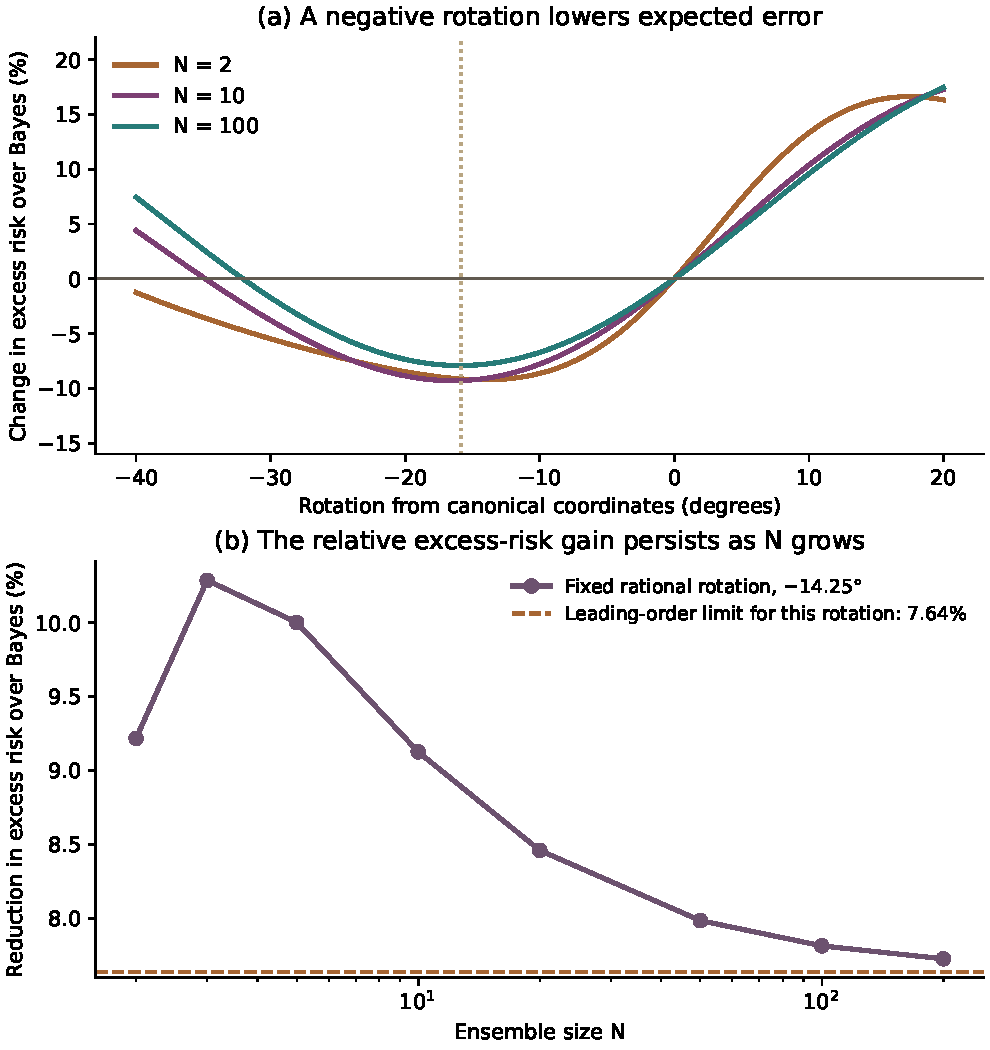
\includegraphics[width=0.78\linewidth]{figures/risk_rotation.pdf}
\caption{Deterministic integration for the example \eqref{eq:example}, ensemble-mean update.
(a)~Change in excess risk over the Bayes risk, relative to the canonical basis, as a function of
the rotation angle, for \(N=2\), 10 and 100; negative values favour the rotation. The dotted line
marks the leading-order optimum \(\theta_*\). (b)~Reduction in excess risk for the fixed rotation
\(Q_{\rm num}\) against \(N\); the dashed line is the leading-order limit for \(Q_{\rm num}\), 7.64\%
(the leading-order optimum \(\theta_*\) would give 7.73\%). The rotated column of
Table~\ref{tab:numeric} uses the same rotation.}
\label{fig:rotation}
\end{figure}

The total-risk gain shrinks like \(1/N\) because every method approaches the Bayes risk, but
the relative gain in excess risk stays near 8\%. The next section shows that in a realistic
configuration the excess-risk gain is far larger.

% =====================================================================
\section{Snyder and Hakim's one-dimensional testbed, reconstructed}\label{sec:application}
% =====================================================================

Snyder and Hakim's evidence for their conjecture comes from a one-dimensional example
\cite[Section~4, Figs~3 and~5]{SnyderHakim2022}. We rebuild that setting from their text and
evaluate it with the objective \(F\) of Theorem~\ref{thm:expansion} and by Monte Carlo. This is a
\emph{reconstruction}, not a replication of their figures: their code is not available to us, the
correlation scale is partly illegible in the published text, and several details (grid
placement, observation positions, boundary treatment) had to be inferred.
Table~\ref{tab:sh-setup} lists the choices; Section~\ref{sec:sh-limits} reports the sensitivity
to them.

\begin{table}[ht]
\centering
\caption{Reconstructed setting. ``SH'' marks a value stated in
\cite[Section~4]{SnyderHakim2022}; ``ours'' marks a choice we made where the text leaves it
open.}
\label{tab:sh-setup}
\small
\begin{tabular}{lll}
\toprule
Item & Value & Source\\
\midrule
State & \(N_x=200\), \(x_i=(i+\tfrac12)/200\) on \((0,1)\), not periodic & SH; placement ours\\
Prior & \(x\sim N(0,P)\), unit variance, Mat\'ern \(\nu=5/2\) & SH\\
Correlation & \((1+s+s^2/3)e^{-s}\), \(s=\sqrt5\,r/\rho\), \(\rho=0.03646\) & SH form; \(\rho\) ours\\
& (correlation exactly \(1/2\) at \(r=0.038\)) & SH: \(1/2\) at \(r=0.038\)\\
Observations & \(N_y=50\) point values, every fourth grid point & SH; offset ours\\
Observation error & independent, unit variance (\(\Rn=I\)) & SH\\
Loss & physical squared error, divided by Kalman-filter MSE & SH Figs~3, 5\\
Localisation & complete (diagonal) in each whitening basis & SH Section~3.2\\
\bottomrule
\end{tabular}
\end{table}

In canonical coordinates \(x=Lz\) with \(L=P^{1/2}V\), where \(V\) holds the right singular vectors
of \(\Rn^{-1/2}HP^{1/2}\); the loss weight is \(W=L\T L=V\T PV\). With \(C\), \(B\) and \(A\) as in
Section~\ref{sec:expansion}, every whitening basis is an orthogonal matrix \(U\) acting on \(z\). We
compare four bases:
\begin{itemize}
\item \emph{canonical}: \(U=I\), Snyder and Hakim's Eq.~8;
\item \emph{P-eigen}: the eigenvectors of \(P\), their Eq.~15, which ignore the observations;
\item \emph{ZCA}: symmetric whitening \(P^{-1/2}x\) \cite{Kessy2018}, which keeps each whitened
 variable attached to one grid point;
\item \emph{F-optimised}: the best basis found by Riemannian gradient descent on \(O(200)\) with
 a Cayley retraction, started from both the canonical and the ZCA basis. It is not certified to
 be a global minimiser of \(F\).
\end{itemize}
The two descents end within \(6\times10^{-5}\) of each other in \(F\). After 4000 iterations
neither met the strict gradient tolerance (final Riemannian gradient norm about
\(1.7\times10^{-4}\)), so the reported \(F_{\rm opt}\) is an upper bound on the minimum; its last
1000 iterations changed \(F\) by less than \(0.02\%\).

\subsection{The leading-order objective}

The canonical basis fails the criterion of Theorem~\ref{thm:criterion} on both counts. The
commutator has \(\norm{[W,C]}_F/\norm{WC}_F=0.056\). And, even ignoring the commutator, the
diagonal weights are ordered the wrong way: across canonical directions the loss weights
\(\lambda_i=u_i\T Au_i\) and the information weights \(\mu_i=u_i\T Bu_i\) have correlation
\(+0.88\), whereas \eqref{eq:opposite} asks for an opposite ordering. Table~\ref{tab:sh-F}
gives \(F\).

\begin{table}[ht]
\centering
\caption{Leading objective \(F(U)\) in the reconstructed testbed. ``Spread'' is
\((\sum_i\mu_i)^2/\sum_i\mu_i^2\), the effective number of basis directions that carry observation
information (\(\sum_i\mu_i=\tr B=15.92\) for every basis).}
\label{tab:sh-F}
\small
\begin{tabular}{lrrr}
\toprule
Basis & \(F(U)\) & Spread & \(\max_i\mu_i\)\\
\midrule
Canonical (SH Eq.~8) & 12.004 & 27.3 & 0.81\\
P-eigen (SH Eq.~15) & 12.030 & 27.3 & 0.81\\
Haar-random, exact mean \((\tr A\tr B+2\tr(AB))/(m+2)\) & 2.229 & & \\
\quad sampled mean (40 draws) & \(2.229\pm0.002\) & & \\
\quad \(\tr A\,\tr B/m\) & 2.131 & & \\
ZCA (symmetric whitening) & 2.134 & 198.4 & 0.13\\
F-optimised & 1.963 & 185.6 & 0.12\\
\bottomrule
\end{tabular}
\end{table}

At leading order the canonical basis is close to the worst choice. A Haar-random orthogonal
basis has an \(F\) more than five times smaller, and the best value found is \(84\%\) below
canonical (so the true minimum is at least that far below). The
P-eigen basis is almost indistinguishable from canonical, in agreement with Snyder and Hakim's
Fig.~5. The ZCA basis, which they did not test, is within \(9\%\) of the best value found.

\subsection{Finite-ensemble risk}

For a fixed orthonormal \(U\), complete localisation uses only the sample variances of
\(w=U\T z\). By rotation invariance (Section~\ref{sec:setting}) these are independent
\(\chi^2_\nu/\nu\) variables, independent of the ensemble mean, so the analysis-error covariance
given them is exactly \(a(I-KG)(I-KG)\T+KK\T\) with \(K=M_UG\T(I+GM_UG\T)^{-1}\). We average this
exact conditional risk over 4000 draws per \(N\), using the same draws for every basis so that
paired differences are precise. Table~\ref{tab:sh-mse} and Figure~\ref{fig:sh} report MSE divided
by the Kalman-filter MSE (\(\tr(WC)=63.88\)), as in Snyder and Hakim's figures.

\begin{table}[ht]
\centering
\caption{MSE divided by Kalman-filter MSE, ensemble-mean update. Standard errors are at most
2 in the last digit for canonical and P-eigen at \(N=4\), smaller elsewhere. Brackets: the
leading-order prediction \(1+[\tr(WC^2)/N+2F/(N-1)]/\tr(WC)\). Last column: paired difference,
F-optimised minus canonical, \(\pm\) one standard error.}
\label{tab:sh-mse}
\small
\begin{tabular}{rllllr}
\toprule
\(N\) & Canonical & P-eigen & ZCA & F-optimised & Difference\\
\midrule
4 & 1.366 [1.230] & 1.367 & 1.135 & 1.134 [1.125] & \(-0.2324\pm0.0018\)\\
8 & 1.137 [1.106] & 1.137 & 1.064 & 1.063 [1.061] & \(-0.0743\pm0.0006\)\\
16 & 1.058 [1.051] & 1.058 & 1.031 & 1.031 [1.030] & \(-0.0276\pm0.0002\)\\
32 & 1.027 [1.025] & 1.027 & 1.015 & 1.015 [1.015] & \(-0.0116\pm0.0001\)\\
64 & 1.013 [1.013] & 1.013 & 1.008 & 1.008 [1.008] & \(-0.0054\pm0.0000\)\\
\bottomrule
\end{tabular}
\end{table}

\begin{figure}[ht]
\centering
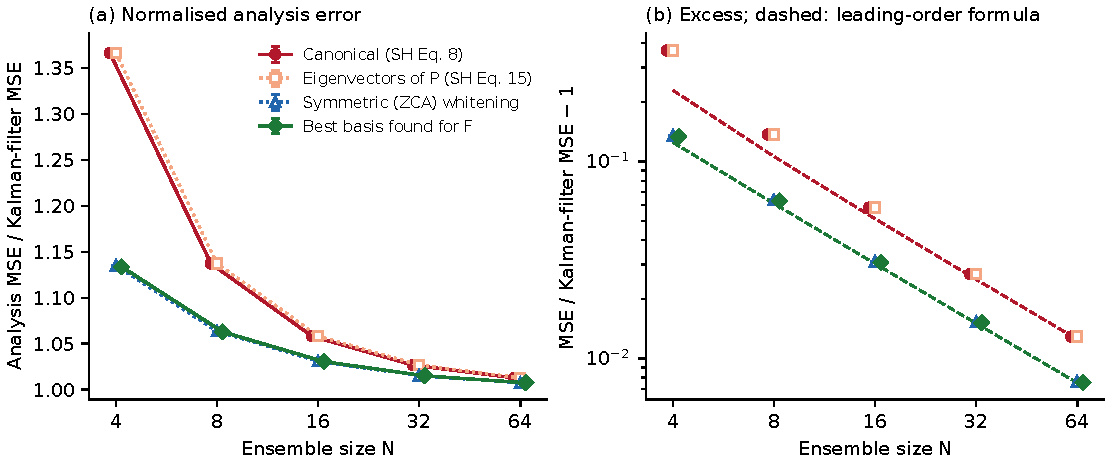
\includegraphics[width=\linewidth]{figures/sh_testbed_mse.pdf}
\caption{Reconstructed Snyder--Hakim testbed: analysis MSE divided by Kalman-filter MSE for
complete localisation in four whitening bases; one analysis, oracle prior covariance.
(a)~Normalised MSE; error bars are \(\pm2\) standard errors, mostly smaller than the markers.
P-eigen overlies canonical, and ZCA overlies the F-optimised basis. (b)~The same results as
excess over the Kalman filter on log axes; dashed lines are the leading-order formula of
Theorem~\ref{thm:expansion}.}
\label{fig:sh}
\end{figure}

The F-optimised basis removes \(54\%\) of the canonical basis's excess error over the Kalman
filter at \(N=8\), \(47\%\) at \(N=16\) and \(42\%\) at \(N=64\). In Snyder and Hakim's units that is
7.4\% of Kalman-filter MSE at \(N=8\) and 2.8\% at \(N=16\). The gap between canonical and P-eigen
is \(+0.01\%\) of Kalman-filter MSE, with a paired standard error of \(2\times10^{-6}\). The
known-mean update gives the same picture: \(1.071\) against \(1.009\) at \(N=8\). The leading-order
formula is accurate for the spread-out bases from \(N=8\), and for canonical from \(N=32\). At small
\(N\) it understates the canonical risk, so the leading order is conservative about the size of the
failure.

\emph{Equivalent ensemble size.} Interpolating the F-optimised risk curve, its risk at
\(N_{\rm eq}\) matches canonical at \(N\) for \((N,N_{\rm eq})=(8,3.9)\), \((16,8.6)\), \((32,18.3)\)
and \((64,37.5)\); the ZCA values are within \(0.5\) of these. In this setting canonical
localisation needs roughly \(1.7\) to \(2\) times as many members as symmetric whitening to reach
the same analysis error.

\emph{Mechanism.} The canonical basis concentrates all observation information into the 50
observed directions: its \(\mu_i\) range up to \(0.81\), with an effective spread of 27 directions.
The same directions carry most of the loss weight \(\lambda_i\). Each localised variance has
relative sampling error \(\sqrt{2/\nu}\), and Theorem~\ref{thm:expansion} prices that error at
\(\lambda_i\mu_i\), so putting large \(\lambda\) and large \(\mu\) in the same directions maximises
the cost. The F-optimised basis spreads the same total information \(\tr B\) over about 186
directions, none with \(\mu_i>0.12\), and reverses the ordering: the correlation of \(\lambda_i\)
and \(\mu_i\) becomes \(-0.96\). Each optimised vector keeps between \(12\%\) and \(61\%\) of its weight
in the observed canonical block (median \(19\%\)), so it mixes observed with unobserved canonical
directions, as Theorem~\ref{thm:criterion} and Corollary~\ref{cor:obsunobs} suggest. Symmetric
whitening achieves almost the same spreading without any optimisation, because each of its
variables is tied to one grid point. Any basis not aligned with the canonical directions does
nearly as well: a single Haar-random basis gives \(1.064\) at \(N=8\).

\emph{Prior-normalised loss.} With \(W=I\) (Mahalanobis loss in \(x\)) the same testbed behaves as
Theorem~\ref{thm:criterion} predicts. The canonical basis is stationary for \(F\), with a gradient
that is exactly zero. Descents started from ZCA, P-eigen and two Haar-random bases all end at or
above canonical: the best reaches \(3.60869\), against \(F_{\rm can}=3.60866\). The Monte Carlo
agrees. ZCA is now worse than canonical by \(0.0159\) (\(N=8\)) and \(0.0037\) (\(N=32\)) of the
Kalman-filter risk, and P-eigen is worse by \(5\times10^{-5}\). The choice of loss, not the
testbed, decides which basis is better.

\emph{Estimated bases.} The bases above use the true \(P\). To see how much of the gain survives
estimation, we built each basis from an independent pilot sample of size \(N_p\), with the pilot
covariance Gaspari--Cohn localised and a ridge \(\delta I\) added. The analysis ensembles were
then simulated in physical space, because estimated whitening leaves the transformed variables
correlated and the rotation-invariance shortcut no longer applies. At \(N=8\) the oracle values in this physical-space simulation (800 replicates; compare
Table~\ref{tab:sh-mse}) are 1.136 (canonical), 1.064 (ZCA) and 1.063 (F-optimised). One pilot
draw per configuration gives:
\begin{itemize}
\item \(N_p=200\), GC half-width \(0.2\), \(\delta=10^{-6}\): estimated ZCA \(1.068\) and estimated
 F-optimised \(1.067\). These keep \(93\%\) and \(95\%\) of the oracle gain at \(N=8\), and \(70\%\) and
 \(72\%\) at \(N=16\).
\item \(N_p=200\), GC half-width \(0.2\), \(\delta=10^{-4}\): estimated ZCA and F-optimised keep \(53\%\)
 and \(37\%\) of the oracle gain at \(N=8\); at \(N=16\) ZCA keeps \(8\%\) and estimated F-optimised is
 \emph{worse} than oracle canonical (\(-28\%\) of the gain). So \(\delta=10^{-6}\) is the best of the
 \(N_p=200\) settings tried, not the only one.
\item \(N_p=50\): the best regularisation tried (\(\delta=10^{-4}\)) keeps about \(60\%\) at \(N=8\) but
 none at \(N=16\). With \(\delta=10^{-6}\) both spread-out bases are worse than oracle canonical.
\item Heavier regularisation (half-width \(0.1\), \(\delta=10^{-3}\)): estimated ZCA and F-optimised
 are \(0.12\) to \(0.26\) of Kalman-filter MSE \emph{worse} than canonical at both sample sizes.
\item An unregularised pilot with \(N_p=2000\) recovers essentially all of the gain (estimated ZCA
 \(1.064\), F-optimised \(1.063\) at \(N=8\)).
\item Estimated \emph{canonical} is robust: within \(0.008\) (\(N_p=200\)) and \(0.031\) (\(N_p=50\)) of
 oracle canonical at \(N=8\), for every regularisation tried.
\end{itemize}
Random estimation error in the whitening is harmless, since nearly any basis not aligned with
canonical does well. Systematic distortion is not. About 100 eigenvalues of \(P\) lie below
\(10^{-3}\) (the smallest is \(2.9\times10^{-5}\)), and a ridge or taper that inflates them leaves
the spread-out coordinates strongly correlated, so complete localisation discards real
covariance. Canonical localisation depends only on the 50 observed, large-scale directions,
which are well estimated. In this testbed the oracle gain is real but fragile in practice.
Turning it into a scheme needs a whitening that is accurate in the small-variance directions,
or a basis chosen to be robust to their misestimation; this matches Snyder and Hakim's remark
that the optimal transformation does not lead directly to practical schemes.

\subsection{The homogeneous (Fourier) case}

Snyder and Hakim single out the homogeneous case, with uniform observations and homogeneous
errors, as the one where the optimal transformation is known analytically: the discrete
Fourier transform \cite[Section~7]{SnyderHakim2022}. Under physical loss
Theorem~\ref{thm:criterion} shows that it is generally not leading-order optimal.

\begin{corollary}[Fourier bases under physical loss]\label{cor:fourier}
Let \(P\) be circulant with mode variances \(p_i>0\), \(H=I\) and \(\Rn=\sigma^2I\), \(\sigma>0\). The
Fourier basis is canonical, with \(W=\diag(p_i)\), \(c_i=\sigma^2/(\sigma^2+p_i)\),
\(\lambda_i=c_i^2p_i=\sigma^4p_i/(\sigma^2+p_i)^2\) and \(\mu_i=p_i/(\sigma^2+p_i)\). If two modes satisfy
\(p_j<p_i\le\sigma^2\), the Fourier basis does not minimise \(F\): a \(45^\circ\) mixing of those two
modes lowers \(F\) by \((\lambda_i-\lambda_j)(\mu_i-\mu_j)/2>0\).
\end{corollary}
\begin{proof}
Here \(W\) and \(C\) are both diagonal in the Fourier basis, so they commute. The maps
\(p\mapsto\mu\) and \(p\mapsto\lambda\) are both strictly increasing on \((0,\sigma^2]\), since
\(\frac{d}{dp}\,p/(\sigma^2+p)^2=(\sigma^2-p)/(\sigma^2+p)^3\). Hence
\((\lambda_i-\lambda_j)(\mu_i-\mu_j)>0\), violating \eqref{eq:opposite}, and the \(45^\circ\)
reduction is the one computed in the proof of Theorem~\ref{thm:criterion}.
\end{proof}

The commutation condition holds here, and only the ordering fails, so the two conditions of
Theorem~\ref{thm:criterion} are independent. Numerically we used a periodic 64-point grid with
the same Mat\'ern correlation and \(\sigma^2=1\). The real Fourier basis diagonalises \(P\) to
\(10^{-14}\), and 47 of the 64 modes have \(p_i<\sigma^2\). Every one of the 1058 distinct pairs
below \(\sigma^2\) violates the ordering, and so do 671 further pairs. The predicted and computed
\(45^\circ\) reductions agree to \(10^{-15}\), and descent from a perturbed Fourier basis lowers \(F\)
from \(3.08\) to \(1.67\). As a control we set \(\sigma^2\) below every mode variance; then no pair
violates the ordering and the Fourier basis is leading-order optimal, as the corollary requires.
The same test applies to any spectral or wavelet-diagonal localisation: under physical loss it is
leading-order optimal only if loss weight and information are oppositely ordered across its
modes.

\subsection{Limits of the reconstruction}\label{sec:sh-limits}

\begin{itemize}
\item \emph{Oracle basis.} The F-optimised and ZCA bases use the true \(P\). The estimated-basis
 test shows that the gain survives only with careful, regularisation-dependent estimation, and
 it used one pilot draw per configuration.
\item \emph{One analysis, Gaussian ensemble.} There is no cycling, no model error and no
 inflation. Complete localisation is compared with complete localisation; tuned
 Gaspari--Cohn localisation in physical space is not part of this comparison.
\item \emph{Reconstruction uncertainty.} Our calibrated \(\rho=0.0365\) gives correlation \(1/2\) at
 exactly \(r=0.038\); the two readings \(\sqrt2/40\) and \(1.5/40\) of the partly illegible scale give
 \(r=0.037\) and \(0.039\), inside our sensitivity range. Changing \(\rho\) by factors \(0.5\) and
 \(1.5\), or \(N_y\) to 25 or 100, leaves the conclusion unchanged: canonical \(F\) stays 4 to 8
 times the best value found, and at \(N=8\) the F-optimised basis improves MSE/KF-MSE by \(0.059\) to
 \(0.077\) (all paired \(z>60\)).
\item \emph{Comparison with Snyder and Hakim's Fig.~5.} They report canonical better than
 P-eigen by more than \(0.5\%\) of Kalman-filter MSE for \(N\le16\); we find \(0.01\%\). For one
 Gaussian realisation the relative standard deviation of the squared error at Kalman-filter
 accuracy is \(0.27\), so an average over 800 unpaired realisations has a standard error near
 \(1\%\) of Kalman-filter MSE. Differences of their size are within that sampling noise, but we
 cannot tell from the text whether their comparison was paired.
\item \emph{Optimiser.} \(F_{\rm opt}\) is an upper bound on the minimum over \(O(200)\); a better
 optimiser could only strengthen the contrast.
\end{itemize}

% =====================================================================
\section{Discussion}\label{sec:discussion}
% =====================================================================

\subsection{What the results mean in practice}

\emph{Population diagonalisation is not the same as estimation-risk minimisation.} Canonical
coordinates remain the right way to \emph{describe} the Gaussian update: they decouple it
exactly. Choosing a basis for \emph{localisation} is a different problem, because it trades
sampling error against the loss used to judge the analysis. In the reconstructed testbed,
under physical squared error, the canonical basis concentrates observation information in the
directions that also carry the most loss weight, which is exactly where sampling error in the
variances does most damage. Physical loss alone does not imply this: Theorem~\ref{thm:criterion}
decides it, and Remark~\ref{rem:physok} gives a case where canonical coordinates are
leading-order optimal under physical loss.

\emph{A loss-aware basis.} The leading objective \(F(U)=\sum_i(u_i\T Bu_i)(u_i\T Au_i)\) uses the
same ingredients as the canonical transformation (\(P\), \(H\), \(R\)) plus the loss. It gives a
computable rule for choosing a complete-localisation basis, and Theorem~\ref{thm:criterion} says
when canonical coordinates are already optimal. A practical reading, when the prior covariance
is accurately known, is: choose the whitening basis with the loss in mind, and check the
criterion before relying on canonical coordinates.

\emph{Simple bases do well.} In the reconstructed testbed, plain symmetric (ZCA) whitening, which
needs no singular value decomposition and is cheaper than the canonical transformation, comes
within \(9\%\) of the best \(F\) found and within \(0.002\) of the finite-\(N\) risk of the best basis
found at every \(N\) tested. Its advantage over canonical localisation is equivalent to roughly
doubling the ensemble. With the prior covariance known, the message for this testbed is that
canonical coordinates are a poor choice before complete localisation and that no fine-tuned
rotation is needed to do much better; with an estimated covariance the advantage is fragile
(below).

\emph{When canonical coordinates are right.} Under prior-normalised loss the canonical basis is
leading-order optimal for every observation network, within the class stated after
Theorem~\ref{thm:criterion}, and, for a scalar observation, a strict local minimum at finite \(N\)
in every case we computed. If a system is judged by a Mahalanobis-type metric, Snyder and Hakim's
choice is the right target.

\emph{Estimation is the main barrier.} With an estimated prior covariance, the advantage of the
spread-out bases survived only with accurate estimation of the small-variance directions;
heavy regularisation reversed it. Canonical localisation was robust to estimation.

\subsection{Limits}

The theory concerns one analysis step with an independent Gaussian forecast ensemble and an
oracle prior covariance used to build every basis. The comparison classes are deterministic
tapers; sample-adaptive corrections \cite{Anderson2012}, shrinkage, hybrid covariances and
tuned distance-based localisation are outside them. The exact all-\(N\) taper comparison is for a
scalar observation; with several observations the finite-\(N\) obstruction is against rotated
complete localisations, and the comparison with all canonical tapers is asymptotic
(Corollary~\ref{cor:largeN}). The expansion holds for fixed dimensions, whereas operational
systems have \(m\gg N\). No real observations, forecast model or cycling were tested, and the
testbed is a reconstruction with the uncertainties listed in Section~\ref{sec:sh-limits}.

\subsection{Open problems}

\begin{enumerate}
\item \emph{Prior-normalised loss at finite \(N\).} Prove \(\zeta_{\nu,a,\beta}>0\)
 (Open problem~\ref{op:WI}), and decide whether canonical complete localisation is globally
 optimal under \(W=I\) at finite \(N\), for scalar and for vector observations.
\item \emph{Two observed directions.} Prove Conjecture~\ref{conj:phisign}, which would make
 \([W,C]=0\) necessary and sufficient for finite-\(N\) stationarity.
\item \emph{Estimated bases.} Find a data-driven estimator of a loss-aware basis that is robust
 to misestimation of small prior variances, and quantify the loss relative to the oracle.
\item \emph{Cycling.} Determine whether the one-step advantage persists, grows or disappears
 when the forecast covariance is itself propagated from an ensemble.
\item \emph{Joint taper and rotation.} Optimise the basis and a partial (not complete) taper
 jointly, including inflation, rather than comparing complete localisations.
\item \emph{Ties and higher order.} Characterise the \(N^{-2}\) term that decides the comparison
 when the leading objective ties (Remark~\ref{rem:alignedN}), and prove the
 \(O(\nu^{-2})\) remainder sketched in Remark~\ref{rem:sharper}.
\item \emph{High dimension.} Develop the analogue of \(F\) in a proportional regime \(m\sim N\).
\end{enumerate}

\section*{Reproducibility and assurance}
\addcontentsline{toc}{section}{Reproducibility and assurance}

The proofs in this paper are written out in full but have not been machine-verified. Two kinds
of computational evidence are kept separate. \emph{Exact arithmetic}
(\texttt{exact\_certificates.py}, Python fractions) checks the finite constants used in the
proofs: the polynomial certificate \(460/773\), the curvature bounds \(-56/773\) and \(-508/773\),
the second-derivative bound \(H_0=23148\) and the rational rotation certificates.
\emph{Floating-point computations} (\texttt{numerical\_checks.py}, \texttt{theory\_checks.py},
\texttt{sh\_testbed.py}) evaluate expectations by deterministic quadrature and by seeded Monte
Carlo, including a Monte Carlo of the actual ensemble procedure with \(4\times10^6\) ensembles that
checks Lemma~\ref{lem:taper}, Theorem~\ref{thm:gradient}, the inflation-robust derivative,
Proposition~\ref{prop:curvature} and two Table~\ref{tab:numeric} entries within stated standard errors, together with negative controls that
must fail. Floating-point results are illustrations and consistency checks, not interval
certificates. Every script records its own SHA-256 hash, writes to a new output directory and
exits with an error if any check fails. The paper received internal, AI-assisted review only; it
has not been externally peer reviewed. The literature search behind the novelty statement was
bounded and is dated 3~November~2026; it is not a certificate of priority.

This is version 0.2.0-candidate, an unrefereed research candidate. It corrects version
0.1.0-candidate (doi:10.5281/zenodo.23926884) only in how it cites Furrer and Bengtsson
\cite{FurrerBengtsson2007}. Their paper has now been compared in full with this one, and
Section~\ref{sec:relation} states what it already contains. No theorem, proof, computation or
recorded output has changed. The paper, its \LaTeX{} source, the
scripts and their recorded outputs are archived at
\href{https://doi.org/10.5281/zenodo.23941881}{doi:10.5281/zenodo.23941881} (all versions:
\href{https://doi.org/10.5281/zenodo.23926883}{doi:10.5281/zenodo.23926883}) and in the repository\newline
\url{https://github.com/ipitchford/canonical-covariance-localisation-failure}.

\appendix
\section{An explicit rational finite-angle certificate}\label{app:rational}

Work with \eqref{eq:example}, with either \(a=1\) or \(a=1+1/N\). The moments of
\(D\sim\chi_\nu^2/\nu\) give
\[
 \E(D-1)^2=\frac2\nu,\quad \E[D(D-1)^2]=\frac2\nu\Bigl(1+\frac4\nu\Bigr),\quad
 \E[D^2(D-1)^2]=\frac2\nu\Bigl(1+\frac{14}\nu+\frac{24}{\nu^2}\Bigr).
\]
Cauchy--Schwarz therefore yields
\[
 \E\frac{(D-1)^2}{(1+D)^2}\ge\frac{(\E(D-1)^2)^2}{\E[(D-1)^2(1+D)^2]}=\frac{\nu}{2\nu^2+11\nu+12},
\]
and since \(\gamma_{\nu,a,1}\ge\E[(D-1)^2(1+D)^{-2}]\) (proof of Theorem~\ref{thm:gradient}),
\[
 \risk_N'(0)\ge g_\nu:=\frac{2\nu}{2\nu^2+11\nu+12}.
\]
For \(\nu=2\) and \(\nu=3\) this gives the same value \(2/21\).

Next, a second-derivative bound valid for every angle. Put \(\Sigma=D_1+D_2\). For the rotated
covariance and gain,
\(\norm{M_\theta}\le\Sigma\), \(\norm{M_\theta'}\le\Sigma\), \(\norm{M_\theta''}\le2\Sigma\), and
differentiating \(k=M_\theta e_1/(1+(M_\theta)_{11})\) gives
\(\norm k\le\Sigma\), \(\norm{k'}\le\Sigma(1+\Sigma)\), \(\norm{k''}\le2\Sigma(1+\Sigma)^2\). Since
\(\norm W=(3+\sqrt5)/2<3\) and \(a\le3/2\),
\[
 |\risk_N''(\theta)|\le18\,\E[\Sigma(1+\Sigma)^2]+45\,\E[\Sigma^2(1+\Sigma)^2].
\]
\(\Sigma\) is gamma distributed with shape \(\nu\) and scale \(2/\nu\); for \(\nu\ge1\) its first four
moments are at most \(2,8,48,384\). Thus
\(|\risk_N''(\theta)|\le18\cdot66+45\cdot488=23148=:H_0\) for all \(\theta\). Set
\[
 t_\nu=\frac{g_\nu}{4H_0},\qquad
 Q_\nu=\frac1{1+t_\nu^2}\begin{pmatrix}1-t_\nu^2&2t_\nu\\-2t_\nu&1-t_\nu^2\end{pmatrix}.
\]
Its entries are rational, and it rotates through \(-\delta_\nu=-2\arctan t_\nu\) with
\(t_\nu\le\delta_\nu\le2t_\nu\). Taylor's theorem gives
\[
 \risk_N(Q_\nu)-\risk_N(I)\le-g_\nu\delta_\nu+\tfrac12H_0\delta_\nu^2\le-\frac{g_\nu^2}{8H_0}<0 .
\]
For \(\nu=2\) this is \eqref{eq:exactgap}.

\section{Evaluating the expectations numerically}\label{app:numerics}

For \eqref{eq:example}, write \(u=\cos^2\!\theta\,D_1+\sin^2\!\theta\,D_2\),
\(v=\cos\theta\sin\theta\,(D_1-D_2)\) and \(k=(u,v)\T/(1+u)\). The direct calculation integrates
\eqref{eq:risk} over independent gamma variables \(D_1,D_2\) (shape \(\nu/2\), scale \(2/\nu\)) with a
tensor generalised Gauss--Laguerre rule. The separate Laplace calculation uses
\((1+u)^{-1}=\int_0^\infty e^{-t}e^{-tu}\,dt\) and \((1+u)^{-2}=\int_0^\infty te^{-t}e^{-tu}\,dt\).
With \(k_\nu=\nu/2\),
\(r_1=(1+t\cos^2\!\theta/k_\nu)^{-1}\), \(r_2=(1+t\sin^2\!\theta/k_\nu)^{-1}\) and
\(\phi(t)=(r_1r_2)^{k_\nu}\),
\begin{gather*}
 \E[e^{-tu}]=\phi(t),\qquad \E[(D_1-D_2)e^{-tu}]=\phi(t)(r_1-r_2),\\
 \E[(D_1-D_2)^2e^{-tu}]=\phi(t)\Bigl[(r_1-r_2)^2+\frac{r_1^2+r_2^2}{k_\nu}\Bigr],
\end{gather*}
so every first and second moment of the gain reduces to one-dimensional integrals. The two
methods agree to within \(5\times10^{-14}\) over 32 comparisons. Both rest on \eqref{eq:risk} and
\eqref{eq:coupling}, so their agreement checks the quadrature and its implementation; the model
itself is checked by the Monte Carlo of the real ensemble procedure described in the
reproducibility statement. The analytic theorems do not depend on any quadrature tolerance.

\bibliographystyle{plainnat}
\bibliography{refs}

\end{document}
